\documentclass[twoside]{article}

\usepackage{aistats2024}

\usepackage{aux/amirhesam_macros}
% If your paper is accepted, change the options for the package
% aistats2024 as follows:
%
%\usepackage[accepted]{aistats2024}
%
% This option will print headings for the title of your paper and
% headings for the authors names, plus a copyright note at the end of
% the first column of the first page.

% If you set papersize explicitly, activate the following three lines:
%\special{papersize = 8.5in, 11in}
%\setlength{\pdfpageheight}{11in}
%\setlength{\pdfpagewidth}{8.5in}

% If you use natbib package, activate the following three lines:
\usepackage[round]{natbib}
\renewcommand{\bibname}{References}
\renewcommand{\bibsection}{\subsubsection*{\bibname}}

% If you use BibTeX in apalike style, activate the following line:
%\bibliographystyle{apalike}

% Optional math commands from https://github.com/goodfeli/dlbook_notation.
%%%%% NEW MATH DEFINITIONS %%%%%

\usepackage{amsmath,amsfonts,bm}

% Mark sections of captions for referring to divisions of figures
\newcommand{\figleft}{{\em (Left)}}
\newcommand{\figcenter}{{\em (Center)}}
\newcommand{\figright}{{\em (Right)}}
\newcommand{\figtop}{{\em (Top)}}
\newcommand{\figbottom}{{\em (Bottom)}}
\newcommand{\captiona}{{\em (a)}}
\newcommand{\captionb}{{\em (b)}}
\newcommand{\captionc}{{\em (c)}}
\newcommand{\captiond}{{\em (d)}}

% Highlight a newly defined term
\newcommand{\newterm}[1]{{\bf #1}}


% Figure reference, lower-case.
\def\figref#1{figure~\ref{#1}}
% Figure reference, capital. For start of sentence
\def\Figref#1{Figure~\ref{#1}}
\def\twofigref#1#2{figures \ref{#1} and \ref{#2}}
\def\quadfigref#1#2#3#4{figures \ref{#1}, \ref{#2}, \ref{#3} and \ref{#4}}
% Section reference, lower-case.
\def\secref#1{section~\ref{#1}}
% Section reference, capital.
\def\Secref#1{Section~\ref{#1}}
% Reference to two sections.
\def\twosecrefs#1#2{sections \ref{#1} and \ref{#2}}
% Reference to three sections.
\def\secrefs#1#2#3{sections \ref{#1}, \ref{#2} and \ref{#3}}
% Reference to an equation, lower-case.
\def\eqref#1{equation~\ref{#1}}
% Reference to an equation, upper case
\def\Eqref#1{Equation~\ref{#1}}
% A raw reference to an equation---avoid using if possible
\def\plaineqref#1{\ref{#1}}
% Reference to a chapter, lower-case.
\def\chapref#1{chapter~\ref{#1}}
% Reference to an equation, upper case.
\def\Chapref#1{Chapter~\ref{#1}}
% Reference to a range of chapters
\def\rangechapref#1#2{chapters\ref{#1}--\ref{#2}}
% Reference to an algorithm, lower-case.
\def\algref#1{algorithm~\ref{#1}}
% Reference to an algorithm, upper case.
\def\Algref#1{Algorithm~\ref{#1}}
\def\twoalgref#1#2{algorithms \ref{#1} and \ref{#2}}
\def\Twoalgref#1#2{Algorithms \ref{#1} and \ref{#2}}
% Reference to a part, lower case
\def\partref#1{part~\ref{#1}}
% Reference to a part, upper case
\def\Partref#1{Part~\ref{#1}}
\def\twopartref#1#2{parts \ref{#1} and \ref{#2}}

\def\ceil#1{\lceil #1 \rceil}
\def\floor#1{\lfloor #1 \rfloor}
\def\1{\bm{1}}
\newcommand{\train}{\mathcal{D}}
\newcommand{\valid}{\mathcal{D_{\mathrm{valid}}}}
\newcommand{\test}{\mathcal{D_{\mathrm{test}}}}

\def\eps{{\epsilon}}


% Random variables
\def\reta{{\textnormal{$\eta$}}}
\def\ra{{\textnormal{a}}}
\def\rb{{\textnormal{b}}}
\def\rc{{\textnormal{c}}}
\def\rd{{\textnormal{d}}}
\def\re{{\textnormal{e}}}
\def\rf{{\textnormal{f}}}
\def\rg{{\textnormal{g}}}
\def\rh{{\textnormal{h}}}
\def\ri{{\textnormal{i}}}
\def\rj{{\textnormal{j}}}
\def\rk{{\textnormal{k}}}
\def\rl{{\textnormal{l}}}
% rm is already a command, just don't name any random variables m
\def\rn{{\textnormal{n}}}
\def\ro{{\textnormal{o}}}
\def\rp{{\textnormal{p}}}
\def\rq{{\textnormal{q}}}
\def\rr{{\textnormal{r}}}
\def\rs{{\textnormal{s}}}
\def\rt{{\textnormal{t}}}
\def\ru{{\textnormal{u}}}
\def\rv{{\textnormal{v}}}
\def\rw{{\textnormal{w}}}
\def\rx{{\textnormal{x}}}
\def\ry{{\textnormal{y}}}
\def\rz{{\textnormal{z}}}

% Random vectors
\def\rvepsilon{{\mathbf{\epsilon}}}
\def\rvtheta{{\mathbf{\theta}}}
\def\rva{{\mathbf{a}}}
\def\rvb{{\mathbf{b}}}
\def\rvc{{\mathbf{c}}}
\def\rvd{{\mathbf{d}}}
\def\rve{{\mathbf{e}}}
\def\rvf{{\mathbf{f}}}
\def\rvg{{\mathbf{g}}}
\def\rvh{{\mathbf{h}}}
\def\rvu{{\mathbf{i}}}
\def\rvj{{\mathbf{j}}}
\def\rvk{{\mathbf{k}}}
\def\rvl{{\mathbf{l}}}
\def\rvm{{\mathbf{m}}}
\def\rvn{{\mathbf{n}}}
\def\rvo{{\mathbf{o}}}
\def\rvp{{\mathbf{p}}}
\def\rvq{{\mathbf{q}}}
\def\rvr{{\mathbf{r}}}
\def\rvs{{\mathbf{s}}}
\def\rvt{{\mathbf{t}}}
\def\rvu{{\mathbf{u}}}
\def\rvv{{\mathbf{v}}}
\def\rvw{{\mathbf{w}}}
\def\rvx{{\mathbf{x}}}
\def\rvy{{\mathbf{y}}}
\def\rvz{{\mathbf{z}}}

% Elements of random vectors
\def\erva{{\textnormal{a}}}
\def\ervb{{\textnormal{b}}}
\def\ervc{{\textnormal{c}}}
\def\ervd{{\textnormal{d}}}
\def\erve{{\textnormal{e}}}
\def\ervf{{\textnormal{f}}}
\def\ervg{{\textnormal{g}}}
\def\ervh{{\textnormal{h}}}
\def\ervi{{\textnormal{i}}}
\def\ervj{{\textnormal{j}}}
\def\ervk{{\textnormal{k}}}
\def\ervl{{\textnormal{l}}}
\def\ervm{{\textnormal{m}}}
\def\ervn{{\textnormal{n}}}
\def\ervo{{\textnormal{o}}}
\def\ervp{{\textnormal{p}}}
\def\ervq{{\textnormal{q}}}
\def\ervr{{\textnormal{r}}}
\def\ervs{{\textnormal{s}}}
\def\ervt{{\textnormal{t}}}
\def\ervu{{\textnormal{u}}}
\def\ervv{{\textnormal{v}}}
\def\ervw{{\textnormal{w}}}
\def\ervx{{\textnormal{x}}}
\def\ervy{{\textnormal{y}}}
\def\ervz{{\textnormal{z}}}

% Random matrices
\def\rmA{{\mathbf{A}}}
\def\rmB{{\mathbf{B}}}
\def\rmC{{\mathbf{C}}}
\def\rmD{{\mathbf{D}}}
\def\rmE{{\mathbf{E}}}
\def\rmF{{\mathbf{F}}}
\def\rmG{{\mathbf{G}}}
\def\rmH{{\mathbf{H}}}
\def\rmI{{\mathbf{I}}}
\def\rmJ{{\mathbf{J}}}
\def\rmK{{\mathbf{K}}}
\def\rmL{{\mathbf{L}}}
\def\rmM{{\mathbf{M}}}
\def\rmN{{\mathbf{N}}}
\def\rmO{{\mathbf{O}}}
\def\rmP{{\mathbf{P}}}
\def\rmQ{{\mathbf{Q}}}
\def\rmR{{\mathbf{R}}}
\def\rmS{{\mathbf{S}}}
\def\rmT{{\mathbf{T}}}
\def\rmU{{\mathbf{U}}}
\def\rmV{{\mathbf{V}}}
\def\rmW{{\mathbf{W}}}
\def\rmX{{\mathbf{X}}}
\def\rmY{{\mathbf{Y}}}
\def\rmZ{{\mathbf{Z}}}

% Elements of random matrices
\def\ermA{{\textnormal{A}}}
\def\ermB{{\textnormal{B}}}
\def\ermC{{\textnormal{C}}}
\def\ermD{{\textnormal{D}}}
\def\ermE{{\textnormal{E}}}
\def\ermF{{\textnormal{F}}}
\def\ermG{{\textnormal{G}}}
\def\ermH{{\textnormal{H}}}
\def\ermI{{\textnormal{I}}}
\def\ermJ{{\textnormal{J}}}
\def\ermK{{\textnormal{K}}}
\def\ermL{{\textnormal{L}}}
\def\ermM{{\textnormal{M}}}
\def\ermN{{\textnormal{N}}}
\def\ermO{{\textnormal{O}}}
\def\ermP{{\textnormal{P}}}
\def\ermQ{{\textnormal{Q}}}
\def\ermR{{\textnormal{R}}}
\def\ermS{{\textnormal{S}}}
\def\ermT{{\textnormal{T}}}
\def\ermU{{\textnormal{U}}}
\def\ermV{{\textnormal{V}}}
\def\ermW{{\textnormal{W}}}
\def\ermX{{\textnormal{X}}}
\def\ermY{{\textnormal{Y}}}
\def\ermZ{{\textnormal{Z}}}

% Vectors
\def\vzero{{\bm{0}}}
\def\vone{{\bm{1}}}
\def\vmu{{\bm{\mu}}}
\def\vtheta{{\bm{\theta}}}
\def\va{{\bm{a}}}
\def\vb{{\bm{b}}}
\def\vc{{\bm{c}}}
\def\vd{{\bm{d}}}
\def\ve{{\bm{e}}}
\def\vf{{\bm{f}}}
\def\vg{{\bm{g}}}
\def\vh{{\bm{h}}}
\def\vi{{\bm{i}}}
\def\vj{{\bm{j}}}
\def\vk{{\bm{k}}}
\def\vl{{\bm{l}}}
\def\vm{{\bm{m}}}
\def\vn{{\bm{n}}}
\def\vo{{\bm{o}}}
\def\vp{{\bm{p}}}
\def\vq{{\bm{q}}}
\def\vr{{\bm{r}}}
\def\vs{{\bm{s}}}
\def\vt{{\bm{t}}}
\def\vu{{\bm{u}}}
\def\vv{{\bm{v}}}
\def\vw{{\bm{w}}}
\def\vx{{\bm{x}}}
\def\vy{{\bm{y}}}
\def\vz{{\bm{z}}}

% Elements of vectors
\def\evalpha{{\alpha}}
\def\evbeta{{\beta}}
\def\evepsilon{{\epsilon}}
\def\evlambda{{\lambda}}
\def\evomega{{\omega}}
\def\evmu{{\mu}}
\def\evpsi{{\psi}}
\def\evsigma{{\sigma}}
\def\evtheta{{\theta}}
\def\eva{{a}}
\def\evb{{b}}
\def\evc{{c}}
\def\evd{{d}}
\def\eve{{e}}
\def\evf{{f}}
\def\evg{{g}}
\def\evh{{h}}
\def\evi{{i}}
\def\evj{{j}}
\def\evk{{k}}
\def\evl{{l}}
\def\evm{{m}}
\def\evn{{n}}
\def\evo{{o}}
\def\evp{{p}}
\def\evq{{q}}
\def\evr{{r}}
\def\evs{{s}}
\def\evt{{t}}
\def\evu{{u}}
\def\evv{{v}}
\def\evw{{w}}
\def\evx{{x}}
\def\evy{{y}}
\def\evz{{z}}

% Matrix
\def\mA{{\bm{A}}}
\def\mB{{\bm{B}}}
\def\mC{{\bm{C}}}
\def\mD{{\bm{D}}}
\def\mE{{\bm{E}}}
\def\mF{{\bm{F}}}
\def\mG{{\bm{G}}}
\def\mH{{\bm{H}}}
\def\mI{{\bm{I}}}
\def\mJ{{\bm{J}}}
\def\mK{{\bm{K}}}
\def\mL{{\bm{L}}}
\def\mM{{\bm{M}}}
\def\mN{{\bm{N}}}
\def\mO{{\bm{O}}}
\def\mP{{\bm{P}}}
\def\mQ{{\bm{Q}}}
\def\mR{{\bm{R}}}
\def\mS{{\bm{S}}}
\def\mT{{\bm{T}}}
\def\mU{{\bm{U}}}
\def\mV{{\bm{V}}}
\def\mW{{\bm{W}}}
\def\mX{{\bm{X}}}
\def\mY{{\bm{Y}}}
\def\mZ{{\bm{Z}}}
\def\mBeta{{\bm{\beta}}}
\def\mPhi{{\bm{\Phi}}}
\def\mLambda{{\bm{\Lambda}}}
\def\mSigma{{\bm{\Sigma}}}

% Tensor
\DeclareMathAlphabet{\mathsfit}{\encodingdefault}{\sfdefault}{m}{sl}
\SetMathAlphabet{\mathsfit}{bold}{\encodingdefault}{\sfdefault}{bx}{n}
\newcommand{\tens}[1]{\bm{\mathsfit{#1}}}
\def\tA{{\tens{A}}}
\def\tB{{\tens{B}}}
\def\tC{{\tens{C}}}
\def\tD{{\tens{D}}}
\def\tE{{\tens{E}}}
\def\tF{{\tens{F}}}
\def\tG{{\tens{G}}}
\def\tH{{\tens{H}}}
\def\tI{{\tens{I}}}
\def\tJ{{\tens{J}}}
\def\tK{{\tens{K}}}
\def\tL{{\tens{L}}}
\def\tM{{\tens{M}}}
\def\tN{{\tens{N}}}
\def\tO{{\tens{O}}}
\def\tP{{\tens{P}}}
\def\tQ{{\tens{Q}}}
\def\tR{{\tens{R}}}
\def\tS{{\tens{S}}}
\def\tT{{\tens{T}}}
\def\tU{{\tens{U}}}
\def\tV{{\tens{V}}}
\def\tW{{\tens{W}}}
\def\tX{{\tens{X}}}
\def\tY{{\tens{Y}}}
\def\tZ{{\tens{Z}}}


% Graph
\def\gA{{\mathcal{A}}}
\def\gB{{\mathcal{B}}}
\def\gC{{\mathcal{C}}}
\def\gD{{\mathcal{D}}}
\def\gE{{\mathcal{E}}}
\def\gF{{\mathcal{F}}}
\def\gG{{\mathcal{G}}}
\def\gH{{\mathcal{H}}}
\def\gI{{\mathcal{I}}}
\def\gJ{{\mathcal{J}}}
\def\gK{{\mathcal{K}}}
\def\gL{{\mathcal{L}}}
\def\gM{{\mathcal{M}}}
\def\gN{{\mathcal{N}}}
\def\gO{{\mathcal{O}}}
\def\gP{{\mathcal{P}}}
\def\gQ{{\mathcal{Q}}}
\def\gR{{\mathcal{R}}}
\def\gS{{\mathcal{S}}}
\def\gT{{\mathcal{T}}}
\def\gU{{\mathcal{U}}}
\def\gV{{\mathcal{V}}}
\def\gW{{\mathcal{W}}}
\def\gX{{\mathcal{X}}}
\def\gY{{\mathcal{Y}}}
\def\gZ{{\mathcal{Z}}}

% Sets
\def\sA{{\mathbb{A}}}
\def\sB{{\mathbb{B}}}
\def\sC{{\mathbb{C}}}
\def\sD{{\mathbb{D}}}
% Don't use a set called E, because this would be the same as our symbol
% for expectation.
\def\sF{{\mathbb{F}}}
\def\sG{{\mathbb{G}}}
\def\sH{{\mathbb{H}}}
\def\sI{{\mathbb{I}}}
\def\sJ{{\mathbb{J}}}
\def\sK{{\mathbb{K}}}
\def\sL{{\mathbb{L}}}
\def\sM{{\mathbb{M}}}
\def\sN{{\mathbb{N}}}
\def\sO{{\mathbb{O}}}
\def\sP{{\mathbb{P}}}
\def\sQ{{\mathbb{Q}}}
\def\sR{{\mathbb{R}}}
\def\sS{{\mathbb{S}}}
\def\sT{{\mathbb{T}}}
\def\sU{{\mathbb{U}}}
\def\sV{{\mathbb{V}}}
\def\sW{{\mathbb{W}}}
\def\sX{{\mathbb{X}}}
\def\sY{{\mathbb{Y}}}
\def\sZ{{\mathbb{Z}}}

% Entries of a matrix
\def\emLambda{{\Lambda}}
\def\emA{{A}}
\def\emB{{B}}
\def\emC{{C}}
\def\emD{{D}}
\def\emE{{E}}
\def\emF{{F}}
\def\emG{{G}}
\def\emH{{H}}
\def\emI{{I}}
\def\emJ{{J}}
\def\emK{{K}}
\def\emL{{L}}
\def\emM{{M}}
\def\emN{{N}}
\def\emO{{O}}
\def\emP{{P}}
\def\emQ{{Q}}
\def\emR{{R}}
\def\emS{{S}}
\def\emT{{T}}
\def\emU{{U}}
\def\emV{{V}}
\def\emW{{W}}
\def\emX{{X}}
\def\emY{{Y}}
\def\emZ{{Z}}
\def\emSigma{{\Sigma}}

% entries of a tensor
% Same font as tensor, without \bm wrapper
\newcommand{\etens}[1]{\mathsfit{#1}}
\def\etLambda{{\etens{\Lambda}}}
\def\etA{{\etens{A}}}
\def\etB{{\etens{B}}}
\def\etC{{\etens{C}}}
\def\etD{{\etens{D}}}
\def\etE{{\etens{E}}}
\def\etF{{\etens{F}}}
\def\etG{{\etens{G}}}
\def\etH{{\etens{H}}}
\def\etI{{\etens{I}}}
\def\etJ{{\etens{J}}}
\def\etK{{\etens{K}}}
\def\etL{{\etens{L}}}
\def\etM{{\etens{M}}}
\def\etN{{\etens{N}}}
\def\etO{{\etens{O}}}
\def\etP{{\etens{P}}}
\def\etQ{{\etens{Q}}}
\def\etR{{\etens{R}}}
\def\etS{{\etens{S}}}
\def\etT{{\etens{T}}}
\def\etU{{\etens{U}}}
\def\etV{{\etens{V}}}
\def\etW{{\etens{W}}}
\def\etX{{\etens{X}}}
\def\etY{{\etens{Y}}}
\def\etZ{{\etens{Z}}}

% The true underlying data generating distribution
\newcommand{\pdata}{p_{\rm{data}}}
% The empirical distribution defined by the training set
\newcommand{\ptrain}{\hat{p}_{\rm{data}}}
\newcommand{\Ptrain}{\hat{P}_{\rm{data}}}
% The model distribution
\newcommand{\pmodel}{p_{\rm{model}}}
\newcommand{\Pmodel}{P_{\rm{model}}}
\newcommand{\ptildemodel}{\tilde{p}_{\rm{model}}}
% Stochastic autoencoder distributions
\newcommand{\pencode}{p_{\rm{encoder}}}
\newcommand{\pdecode}{p_{\rm{decoder}}}
\newcommand{\precons}{p_{\rm{reconstruct}}}

\newcommand{\laplace}{\mathrm{Laplace}} % Laplace distribution

\newcommand{\E}{\mathbb{E}}
\newcommand{\Ls}{\mathcal{L}}
\newcommand{\R}{\mathbb{R}}
\newcommand{\emp}{\tilde{p}}
\newcommand{\lr}{\alpha}
\newcommand{\reg}{\lambda}
\newcommand{\rect}{\mathrm{rectifier}}
\newcommand{\softmax}{\mathrm{softmax}}
\newcommand{\sigmoid}{\sigma}
\newcommand{\softplus}{\zeta}
\newcommand{\KL}{D_{\mathrm{KL}}}
\newcommand{\Var}{\mathrm{Var}}
\newcommand{\standarderror}{\mathrm{SE}}
\newcommand{\Cov}{\mathrm{Cov}}
% Wolfram Mathworld says $L^2$ is for function spaces and $\ell^2$ is for vectors
% But then they seem to use $L^2$ for vectors throughout the site, and so does
% wikipedia.
\newcommand{\normlzero}{L^0}
\newcommand{\normlone}{L^1}
\newcommand{\normltwo}{L^2}
\newcommand{\normlp}{L^p}
\newcommand{\normmax}{L^\infty}

\newcommand{\parents}{Pa} % See usage in notation.tex. Chosen to match Daphne's book.

\DeclareMathOperator*{\argmax}{arg\,max}
\DeclareMathOperator*{\argmin}{arg\,min}

\DeclareMathOperator{\sign}{sign}
\DeclareMathOperator{\Tr}{Tr}
\let\ab\allowbreak


% packages
\usepackage{xcolor, soul}
\sethlcolor{pink}
\usepackage{array}

% tikz and pgfplots
\usepackage{tikz}
\usepackage{pgfplots}
\usepackage{pgfplotstable}
\pgfplotsset{compat=1.14}
\usepgfplotslibrary[fillbetween,statistics] 
\usepgfplotslibrary{external}
\tikzexternalize[prefix=figuresTikz/] % TODO TODO
\usetikzlibrary{arrows.meta,calc,chains,shapes.geometric}


\usepackage[pagebackref=true]{hyperref}
\hypersetup{
    colorlinks=true,
    citecolor=blue,
    linkcolor=red,
    filecolor=magenta,
    urlcolor=violet}
\renewcommand*\backref[1]{\ifx#1\relax \else (Cited on p. #1) \fi}


\usepackage{forloop}
\usepackage{csvsimple}
\usepackage{booktabs}
\usepackage{caption}
\usepackage{subcaption}
\usepackage{cleveref}
\crefformat{equation}{(#2#1#3)}

\newcounter{rowcount}
\setcounter{rowcount}{0}




% colors
\definecolor{red}{RGB}{215,25,28}
\definecolor{orange}{RGB}{253,174,97}
\definecolor{yellow}{RGB}{255,255,191}
\definecolor{lightblue}{RGB}{171,217,233}
\definecolor{darkblue}{RGB}{44,123,182}
\definecolor{lightgreen}{RGB}{178,223,138}
\definecolor{darkgreen}{RGB}{51,160,44}



\newcommand{\amir}[1]{{\color{purple}\textbf{[Amir:} \textit{#1}\textbf{]}}}
\newcommand{\daniel}[1]{{\color{violet}\textbf{[Daniel:} \textit{#1}\textbf{]}}}
\newcommand{\todo}[1]{{\color{red}\textbf{[TODO:} #1\textbf{]}}}

\newcommand{\V}{\mathbb{V}}
\newcommand{\valpha}{\bm{\alpha}}







\begin{document}





\twocolumn[

% \aistatstitle{\hl{Recursive Feature Learning in Gaussian Processes}}

\aistatstitle{\hl{Uncertainty Estimation with Recursive Feature Machines}}

\aistatsauthor{ Author 1 \And Author 2 \And  Author 3 }

\aistatsaddress{ Institution 1 \And  Institution 2 \And Institution 3 } ]







\begin{abstract}
In conventional regression analyses, predictions are typically represented as point estimates derived from covariates. Gaussian Processes (GP) offer a framework that predicts and in addition, quantifies associated uncertainties. This is particularly crucial in areas like healthcare and weather forecasting, where there is a growing recognition of the importance of capturing uncertainty. However, kernel-based methods are typically outperformed by ensemble decision tree methods on tabular/categorical data sets in downstream regression tasks. In this study, we harness the power of the recently proposed Recursive Feature Machines (RFMs) to enhance feature extraction through kernel methods. We subsequently employ this learned kernel for in-depth uncertainty analysis. Remarkably, when tested on tabular datasets, our RFM-based method consistently surpasses other leading uncertainty estimation techniques, including NGBoost and CatBoost-ensemble. We also demonstrate how our method can be integrated with deep networks and how it performs comparably to deep ensembles.
% In conventional regression analyses, predictions are typically represented as point estimates derived from covariates. However, there is a growing recognition of the importance of capturing uncertainty in predictions, especially in critical domains like healthcare and weather forecasting. Probabilistic regression models, such as Gaussian Processes (GPs), have risen to this challenge by offering a comprehensive probability distribution over the outcome space, contingent on these covariates. GPs Bayesian nature provides a natural avenue for uncertainty quantification.
% In the midst of this evolving landscape, tree ensemble models like XG-boost emerged as state-of-the-art for tabular data. Yet, their major drawback was their inability to encapsulate uncertainty. This gap led to the development of methods like NG-boost and cat-boost, which prioritized uncertainty quantification. The most recent addition to this domain is the Recursive Feature Machine (RFM) kernel-based model, renowned for its exceptional feature learning capabilities. Specifically, for tabular datasets, it has demonstrated superior performance over fully connected networks and has either matched or surpassed the capabilities of XG-boost.
% In this study, we leverage the capabilities of RFMs to enhance feature extraction through kernel methods and subsequently employ this learned kernel for rigorous uncertainty analysis. Our empirical results on tabular datasets, reveal that the RFM-based approach consistently outshines other leading uncertainty estimation techniques, including NG-boost and cat-boost. Additionally, we conduct experiments to demonstrate how our method can seamlessly integrate with deep networks and perform comparably to deep ensemble methods, suggesting a promising direction for future research and applications.
\end{abstract}








\section{INTRODUCTION}

Regression analyses have long been the bedrock of predictive modelling, where the primary goal is to forecast future outcomes based on historical data. In its conventional form, these predictions are often distilled down to singular, definitive values, which are derived from a set of influencing factors or covariates. However, as the applications of predictive modelling have grown more diverse and complex, especially in critical sectors like healthcare and weather forecasting, there is an increasing realization that a mere point prediction is not sufficient. Stakeholders in these sectors often need to gauge the level of confidence or uncertainty associated with these predictions.

In the rapidly changing realm of machine learning, the recent emergence of Recursive Feature Machines (RFMs) has captured the attention of both researchers and practitioners. RFMs, being kernel-based methods, offer a fresh perspective on extracting and interpreting features from data. Our study delves deeply into the capabilities of RFMs, from their effectiveness in refining predictions to their aptitude in uncertainty estimations. We also evaluate how they compare against other leading techniques, especially the newer decision tree-based methods like NGBoost and CatBoost. 


Meanwhile, Gaussian Processes (GP) have long been the preferred method for assessing uncertainty in predictions, offering a nuanced approach that goes beyond simple point estimates. Yet, with the continuous advancements in machine learning, decision tree-based techniques like NGBoost and CatBoost are making their mark. These methods not only rival GP in prediction accuracy but have also demonstrated superior performance on specific uncertainty metrics such as NLL, coverage, and RMSE, particularly for tabular or categorical data. Emphasizing the importance of ongoing assessment and evolution in the domain, our research also delves into the intrinsic relationship between RFM and traditional GP.

Additionally, we demonstrate how RFM can be integrated with the learned embeddings from Neural Networks, delivering uncertainty estimations comparable to those of NN ensembles. This presents a cost-effective alternative, circumventing the need to train multiple Neural Network models.

% But the world of machine learning is ever-evolving, and the recent introduction of Recursive Feature Machines (RFMs) has stirred interest among researchers and practitioners. RFMs promise to enhance the way we extract and interpret features from data, especially when using kernel methods, which are techniques used to find patterns in data. In this research, we embark on a deep dive into the capabilities and potential of RFMs. Our exploration spans their efficacy in refining predictions, their prowess in uncertainty estimations, and how they stack up against other leading techniques in the field. Furthermore, in an era where deep learning networks are revolutionizing various domains, we also investigate how RFMs can be seamlessly integrated with these advanced architectures. By doing so, we aim to paint a holistic picture of RFMs, shedding light on their potential to reshape the future of predictive modelling and uncertainty estimation.





\subsection{Main contribution}
In this work, we have the following contributions,

\begin{itemize}
    \item We demonstrate that features learned using the RFM method significantly enhance the uncertainty performance on tabular datasets. Given their ability to produce results that are either comparable to or, in certain instances, surpass state-of-the-art (SOTA) methods, RFM positions itself as the new benchmark for applications that demand precise uncertainty estimation.
    \item We establish that RFM-based methods can be synergized with features derived from neural networks, achieving results that stand shoulder to shoulder with deep ensemble methods. This presents RFM as a viable alternative, especially in scenarios where the computational burden of training multiple deep networks is a concern.
    \item We draw a link between traditional GP techniques and RFM, examining their similarities and differences in comparison.
\end{itemize}
\hl{check if we need this as a subsection.}


\section{PRIOR WORK}


% \begin{itemize}
%     \item NG-boost
%     \item cat-boost
%     \item how can we categorize these different methods, and why people potentially want to prefer one to another
%     \item GP, very general
% \end{itemize}


% \begin{enumerate}
%     \item What is the problem
%     \item Why is it challenging
%     \item what have people done to tackle the problem
%     \item connect to our work
% \end{enumerate}


Numerous uncertainty quantification methods have been proposed in the literature for utilization with tabular data. Here, we focus on discussing flexible methods with state-of-the-art predictive performance.

\paragraph{Gaussian processes}
As a non-parametric, flexible Bayesian regression model, the Gaussian Process (GP) is a well-studied, natural choice for uncertainty quantification \citep{rasmussen2006gaussian}. The GP is characterized by a kernel function as covariance. The crucial challenge is to choose the right kernel as it encodes high-level assumptions about the data. Commonly, the Radial Basis Function (RBF) or Laplace kernel is chosen which has a limited number of parameters to optimize. For more flexibility, the Automatic Relevance Determination (ARD) kernel introduces feature weighting through learnable parameters \citep{mackay1992bayesian,neal1996bayesian}. Instead of utilizing advanced kernels, we can equivalently transform the input and use standard kernels \citep{mackay1998introduction}. Neural networks have been studied as feature extractors \citep{calandra2016manifold,wilson2016deep}, or where the last layer approximates a GP \citep{huang2015scalable,liu2020simple}. Our approach combines both strategies, leveraging the recently proposed Recursive Feature Machine \citep{radhakrishnan2022feature}, which introduces a novel feature-extracting kernel.
% \begin{itemize}
%     \item GPs around for a long time
%     \item why used for UQ: natural with covariance
%     \item different GPs for expressive power
%     \item ARD for feature learning
%     \item neural network as feature extractor
%     \item we use RFMs
% \end{itemize}







\paragraph{Probabilistic boosting}
Boosting-based approaches \citep{freund1995desicion,friedman2001greedy} allow for flexible models, which find widespread application on tabular datasets \citep{shwartz2022tabular,grinsztajn2022tree,mcelfresh2023neural}. Such methods include AdaBoost, XGBoost, LightGBM or CatBoost \citep{chen2016xgboost,ke2017lightgbm,prokhorenkova2018catboost}. For classification problems, most methods have a natural probabilistic interpretation through estimated class probabilities. However, for regression problems, there is no such straightforward concept. Therefore, probabilistic extensions of boosting such as NGBoost, CatBoost-Ensembles \citep{duan2020ngboost,malinin2021uncertainty} or extensions to Random Forests \citep{schlosser2019distributional,shaker2020aleatoric} have been proposed. Notably, when comparing the performance of probabilistic boosting approaches against our GP-RFM, our approach outperforms them across a range of evaluation metrics and datasets.
% \begin{itemize}
%     \item boosting with good predictive performance on tabular data
%     \item history of probabilistic boosting approaches
%     \item Ours: surprisingly outperforms
% \end{itemize}
% 
% XGBoost \citep{chen2016xgboost}
% LightGBM \citep{ke2017lightgbm}
% CatBoost \citep{prokhorenkova2018catboost}
% AdaBoost \citep{freund1995desicion}
% \citep{friedman2001greedy}
%
% Boosting arguably the best method for tabular data \citep{shwartz2022tabular,grinsztajn2022tree,mcelfresh2023neural}
%
% Uncertainty for boosting: NGBoost \citep{duan2020ngboost}, CatBoost-Ensembles \citep{malinin2021uncertainty}, Random Forest-based \citep{schlosser2019distributional,shaker2020aleatoric}










\paragraph{Neural networks}
The ability to learn features from data is a key advantage for the predictive power of neural networks (NN). For uncertainty quantification, Bayesian NNs \citep{mackay1992bayesian,neal1996bayesian} are a natural choice. However, the need for approximate inference methods such as variational inference \citep{graves2011practical,blundell2015weight} or Markov Chain Monte Carlo \citep{welling2011bayesian} makes them computationally expensive. Conversely, the use of Monte Carlo dropout \citep{gal2016dropout} provides less reliable uncertainty estimates \citep{ovadia2019can,gustafsson2020evaluating} than ensembles of NNs \citep{lakshminarayanan2017simple}. Although deep ensembles set the gold standard for NNs, they necessitate training multiple NNs. We leverage the idea of feature learning through the use of RFMs which are intricately linked to features learnt in feedforward NNs. Further, we show that we can combine NNs as feature extractors for our GP-RFM to perform on par with deep ensembles.
% \begin{itemize}
%     \item Feature learning leads to impressive results
%     \item Bayesian NN
%     \item Ensembles
%     \item ours: Feature learning in RFMs connected to NNs
% \end{itemize}

% \section{SUMMARY OF CONTRIBUTIONS}


\section{BACKGROUND}

Most machine learning algorithms focus on estimating the predictive model $f(\vx)=\E[y|\vx]$ from a training dataset $\gD=(\mX,\vy)=\{\vx_i\in\R^d,y_i\in\R\}_{i=1}^n$. However, in many applications, this is not sufficient. We are therefore interested in augmenting point estimates with reliable uncertainty quantification to obtain the predictive distribution $p(f(\vx_\ast)|\vx_\ast,\gD)$ for a new test data point $\vx_\ast$. In our approach, we leverage GPs in conjunction with feature learning kernels through RFMs.



\subsection{Kernel machines}
Kernel machines, \citep{scholkopf2002learning} are non-parametric predictive models. Given training data $\gD$  a kernel machine is a model of the form
\begin{align}\label{eq:representer_thm}
    f(\x) = \sum_{i=1}^n\alpha_i k(\x,\x_i).
\end{align}
Here, $k:\R^d\times \R^d\to\R$ is a positive semi-definite symmetric kernel function \citep{aronszajn1950theory}. According to the representer theorem \citep{kimeldorf1970correspondence}, the unique solution to the infinite-dimensional optimization problem
\begin{align}\label{eq:kernel_regression}
    &\arg\min{f\in\gH} \, \sum_{i=1}^n (f(\x_i)-y_i)^2+\lambda\norm{f}_\gH^2
\end{align}
has the form given in \cref{eq:representer_thm}. Here $\gH$ is the (unique) reproducing kernel Hilbert space (RKHS) corresponding to $k$. It can be seen that $\valpha = (\alpha_1,\ldots,\alpha_n)$ in \cref{eq:representer_thm} is the unique solution to the linear system,
\begin{align}\label{eq:linear_system}
    \left(k(\mX,\mX)+\lambda \mI_n \right)\valpha=\y.
\end{align}





\subsection{Gaussian processes}
To extend kernel machines into a probabilistic framework, we can define a distribution over the predictive function which yields a GP $f \sim \gG\gP(m,k)$ specified by its mean function $m$ and its covariance function. Because of its properties, we utilize the kernel function $k$ as the covariance function in the GP. The posterior predictive distribution of the GP is then given by
\begin{align}
    p(f(\vx_\ast)|\vx_\ast,\gD) &= \gN \left( f(\vx_\ast) , \V[f(\vx_\ast)] \right),
    \label{eq:gp-predictive-distribution}
\end{align}
with the mean as in \cref{eq:representer_thm} and the covariance $\V[f(\vx_\ast)]=k(\vx_\ast,\vx_\ast)-\vk_\ast^\top(\mK+\sigma^2\mI)^{-1}\vk_\ast$. We denote the kernel matrix as $\mK$ with $K_{i,j}=k(\vx_i,\vx_j)$, $\vk_\ast=k(\mX,\vx_\ast)$ and the measurement noise variance as $\sigma^2$.

For the mean function, we choose $m=0$.
The choice of kernel encodes high-level assumptions about the resulting function. We consider an exponential kernel of the form
\begin{align}
    k(\vx,\vz) = \exp\left( g(\vx, \vz) \right).
\end{align}
With $g(\vx,\vz)=-\frac{1}{2\ell^2}\|\vx-\vz\|^2$ we obtain the commonly chosen Radial Basis Function (RBF) kernel. With $g(\vx,\vz)=-\frac{1}{\ell}\|\vx-\vz\|$ we obtain the Laplace kernel.

The parameters $\vtheta$ of the kernel include noise variance $\sigma$ and length scale $\ell$. We can select these parameters in a Bayesian framework using the Negative Log Likelihood (NLL) defined as $-\log p(\vy|\mX,\vtheta)$. Minimizing the NLL can be performed with any optimizer.








\subsection{Recursive Feature Machines}

A fundamental limitation of kernel machines is their reliance on kernel functions that are not adaptive to data. As a result, for certain tasks, kernel machines can significantly underperform compared to neural networks. Recently, RFMs were introduced. A type of kernel machine capable of learning features, making them data-adaptive.

To develop kernel machines that can learn features, RFM integrates a positive semi-definite, symmetric matrix, $\mM$, as a learnable parameter into the kernel function. Specifically, this is suited for kernel functions that depend on the distance between points, such as $k(\vx, \vz) = \phi(\|\vx - \vz\|^2)$ where $ \phi: \R \to \R$ and $ \vx, \vz \in \R^d$. We incorporate the learnable matrix $\mM$ by using the Mahalanobis distance
\begin{align}
    \norm{\vx-\vz}_\mM := \sqrt{(\vx-\vz)^T\mM(\vx-\vz)}.
\end{align}
Therefore, the matrix $\mM$ re-weights the individual features and can incorporate correlation between features, which is the reason why we call it the \emph{feature matrix}.
While any kernel function for $\phi$ can be used, we utilize the Laplace kernel based on the Mahalanobis distance
\begin{align}
    k_\mM(\vx,\vz) := \exp\left(-\frac{1}{\gamma}\norm{\vx-\vz}_\mM\right).
\end{align}
The prediction function corresponding to this kernel is given by
\begin{align}
    f_\mM(\vx) = k_\mM(\vx,\mX)\valpha
    \label{eq:rfm-prediction-function}
\end{align}
with $\valpha = k_\mM(\mX,\mX)^{-1}\vy$. To learn the feature matrix $\mM$ we make use of the proposed idea of the Average Gradient Outer Product (AGOP) from \citet{radhakrishnan2022feature}: We start by initializing $\mM^{(0)}=\mI_d$. Then, at each iteration step $t$ we first solve for the kernel weights $\valpha$ from \cref{eq:rfm-prediction-function} with fixed $\mM$. Second, we update $\mM$ using the AGOP defined as
\begin{align}
    \mM^{(t+1)} = \frac{1}{n}\sum_{i=1}^n \nabla_{\vx}f_{\mM^{(t)}}(\vx_i)\nabla_{\vx}f_{\mM^{(t)}}(\vx_i)^T.
    \label{eq:agop}
\end{align}
Intuitively, RFM prioritises the features that have the most impact on the prediction function. Thus, it learns the presentation most relevant to the underlying task.


\paragraph{Remark:} Another way of feature weighting specifically in GPs is through the extension with Automatic Relevance Determination (ARD) \cite{neal1996bayesian} kernels. The RBF kernel is extended by using $g(\vx,\vz)=-\frac{1}{\ell^2}\norm{\vx-\vz}^2_\mM$ with $\mM^{-1}=\text{diag}([\ell_1^2,\dots,\ell_d^2])$ and similarly for the Laplace kernel. This effectively increases the parameter vector $\vtheta$ learnt by minimizing the NLL in the GP framework.









%%%%%%%%%%%%%%%%%%%%%%%%%%%%%%%%%%%%%%%%%%%%%
% OURS
%%%%%%%%%%%%%%%%%%%%%%%%%%%%%%%%%%%%%%%%%%%%%
\section{METHOD: GP-RFM}
% Introduction to GPs and RFMs:
While GPs are powerful non-parametric models which offer uncertainty quantification, they are limited by their reliance on kernel functions that are not adaptive to data. RFMs are a type of kernel machine capable of learning features, making them data-adaptive.
% Integration of RFMs into GPs:
We propose to integrate RFMs into GPs by replacing the kernel function $k(\vx,\vz)$ with the RFM kernel $k_\mM(\vx,\vz)$.
Since we are using the Laplace kernel within the RFM, we denote the resulting GP as \emph{GP-RFM-Laplace}.

% Mathematical Formulation:
Specifically, we consider a combination of a scale kernel with the RFM kernel to obtain $\sigma_f^2 k_\mM(\vx,\vz)$.
Since we are interested in the predictive distribution, we can set the mean function $m$ of the GP to zero. The resulting predictive distribution is then given by \cref{eq:gp-predictive-distribution} where $f(\vx)$ is given by \cref{eq:rfm-prediction-function}.
% Parameterization:
The parameters of the GP are the feature matrix $\mM$ and the kernel parameters $\vtheta$ consisting of noise variance $\sigma$, length scale $\ell$ as well as scale $\sigma_f$.

% Training:
\paragraph{Training}
We disentangle the training of the GP-RFM-Laplace into two steps.
First, we learn the feature matrix $\mM$ using the recursive iteration between solving for the kernel weights $\valpha$ for \cref{eq:rfm-prediction-function} and updating $\mM$ using the AGOP defined in \cref{eq:agop}.
To learn the kernel weights, we solve the linear system in \cref{eq:linear_system} with a Ridge regularization term for stability to obtain $\valpha = (\mK+\lambda_\alpha\mI_n)^{-1}\vy$.
For the AGOP we need to compute the gradient of the prediction function w.r.t. the inputs $\vx_i$. For the Laplace kernel, there exist closed-form solutions which we make use of \citep{radhakrishnan2022feature}.
Second, we learn the kernel parameters $\vtheta$ by minimizing the NLL with fixed $\mM$.

% Extension: add Ridge regularization to AGOP for M computation
\paragraph{Eliminating spurious correlation}
In many datasets, there exist spurious correlations between features. To avoid overfitting to this spurious correlation, we add a Ridge regularization term to the AGOP in \cref{eq:agop} to obtain
\begin{align}
    \mM^{(t+1)} = \frac{1}{n}\sum_{i=1}^n \nabla_{\vx}f_{\mM^{(t)}}(\vx_i)\nabla_{\vx}f_{\mM^{(t)}}(\vx_i)^T + \lambda_\mM\mI_d.
    \label{eq:agop-ridge}
\end{align}
The Ridge regularization acts in this case as a noise filter by shrinking off-diagonal elements of $\mM$ towards zero.
Therefore, the learnt feature correlation in the off-diagonal elements of $\mM$ is only kept if it is supported by the data, making the model more robust to random variations in the data.

% Uncertainty Quantification:
\paragraph{Uncertainty quantification}
During inference, we can quantify the uncertainty of the GP-RFM-Laplace by computing the predictive variance $\V[f(\vx_\ast)]$ from \cref{eq:gp-predictive-distribution}.
In traditional GPs, we have to choose the kernel function carefully to encode assumptions about the resulting function.
In contrast, the GP-RFM-Laplace is able to learn the features from the data and therefore is more flexible in its assumptions about the resulting function.
While \citet{radhakrishnan2022feature} showed the predictive power of RFMs, we show that the learnt features provide additional insight into the variability or ambiguity of the data which is crucial for uncertainty quantification.

% Implementation Details:
\paragraph{Implementation details}
We implement the GP-RFM-Laplace in PyTorch \citep{paszke2019pytorch}. For the computation of the feature matrix in the first step of the training procedure, we rely on the official implementation by \citet{radhakrishnan2022feature}.
For the GP implementation, we use GpyTorch \citep{gardner2018gpytorch} which provides a modular implementation of GPs in PyTorch. To optimize the GP parameters, we use the Adam optimizer \citep{kingma2014adam} with a cosine annealing learning rate scheduler \citep{loshchilov2016sgdr}.
The hyperparameters we have to select are the learning rate, the Ridge regularization parameters $\lambda_\alpha$ and $\lambda_\mM$ for the solver and the AGOP respectively.
Our code will be made publicly available upon acceptance.
\section{EXPERIMENTS}

% Dataset description
\paragraph{Datasets}
We evaluate our GP-RFM-Laplace on a variety of regression tasks.
Specifically, we use two tabular regression benchmarks with datasets from UCI \citep{asuncion2007uci} and OpenML \citep{vanschoren2014openml} respectively.
For the UCI benchmark we use 7 datasets inspired by \citet{duan2020ngboost} and
for the OpenML benchmark, we utilize the collection of 16 numerical regression datasets by \citet{grinsztajn2022tree}.

% Hyperparameter tuning and preprocessing
\paragraph{Hyperparameter tuning}
We follow the protocol proposed in \citet{hernandez2015probabilistic} for data splitting and hyperparameter tuning.
For the UCI benchmark, we follow \citet{duan2020ngboost} to hold out 10\% of the data as a test set.
For the OpenML benchmark, we follow \citet{grinsztajn2022tree} to hold out 30\% of the data as a test set.
The remaining data is split into a 70\% training set and a 30\% validation set in order to tune the hyperparameters.
We use grid-search over all combinations of hyperparameters and select the best hyperparameters based on the NLL on the validation set.
Details on the hyperparameter search space can be found in the appendix.
Finally, we train the model on the full training set and evaluate it on the test set.
The process is repeated for 20 random seeds and we report the mean and standard deviation of the results.

% Baseline methods
\paragraph{Baselines}
%\begin{itemize}
%    \item GPs: RBF, Laplace, ARD-RBF, ARD-Laplace
%    \item Boosting: NGBoost, CatBoost-Ensemble
%\end{itemize}
We compare our GP-RFM-Laplace to a variety of probabilistic baseline methods.
For GPs, we consider the \emph{RBF} and \emph{Laplace} kernel.
% where we learn the length scale parameter $\ell$ and the noise variance $\sigma$.
Additionally, we compare to the \emph{ARD-RBF} \citep{neal1996bayesian} which is used in many settings and to the \emph{ARD-Laplace} kernel.
% where we learn the length scale parameters $\ell_1,\dots,\ell_d$ and the noise variance $\sigma$.
The latter is a rarely used kernel in GPs but is a natural extension of the Laplace kernel to incorporate feature weighting, learnt through NLL minimization.
% boosting approaches
% NGBoost generalizes gradient boosting to probabilistic regression by treating the parameters of the conditional distribution as targets for a multiparameter boosting algorithm
Furthermore, we consider probabilistic extensions of boosting approaches, which are known to be powerful for predictive tasks.
Firstly, we use \emph{NGBoost} \citep{duan2020ngboost} which learns the parameters of a Gaussian distribution through boosting enhanced with a natural gradient update.
Secondly, we use \emph{CatBoost-Ensemble} \citep{prokhorenkova2018catboost} which uses an ensemble of 10 gradient boosting-based models from which the predictive distribution is obtained by computing statistics of the individual predictions.
% preprocessing
Following \citet{duan2020ngboost}, we standardize features and labels to have zero mean and unit variance for all GP-based methods but not for the boosting-based methods.



% Evaluation metrics
\paragraph{Evaluation metrics}
% RMSE, NLL, 95\% Coverage Error, Interval Length at 95\% Coverage
We are interested in the predictive performance of the models as well as their uncertainty quantification.
Therefore, we evaluate the models on their \emph{root mean squared error (RMSE)} as well as their \emph{NLL} on the test set.
We also require the model uncertainty to be calibrated, i.e. the predictive distribution should reflect the likelihood of prediction errors.
To evaluate calibration, we compute the \emph{95\% coverage error (CE)} which refers to the proportion of data points for which the 95\% prediction interval does not contain the true value.
In order for the model to be well-calibrated, the coverage should be 95\% and the corresponding CE should be zero.
Finally, we evaluate the \emph{interval length (IL)} of the 95\% confidence interval. This measure is important for models with similar CE since a smaller IL indicates a more precise uncertainty quantification.








\subsection{Main results}
Here we present the main results of our experiments.
We compare our GP-RFM-Laplace to all baseline methods on the UCI and OpenML benchmark datasets.
% normalization as datasets have different scales
Since the datasets have different scales, we normalize the resulting metrics to compare methods across datasets.
Specifically, for each dataset, we compute the minimum and maximum of the results across all methods and seeds.
Then, we normalize the results of each method and seed to the range $[0,1]$.
% results reference to figures and tables
The results for the OpenML benchmark are shown in \Cref{fig:main-tabular-benchmark} for NLL, RMSE and CE
using violin plots to show the distribution of the results including a boxplot for the median and quartiles.
The results for the UCI benchmark are shown in the appendix.
Note that the results for IL are omitted as comparing IL across datasets is not meaningful.
Detailed results for each dataset individually can be found in the appendix.

% results summary
We observe that our GP-RFM-Laplace is only outperformed by the CatBoost-Ensemble in terms of NLL.
However, the GP-RFM-Laplace is the best method in terms of RMSE, closely followed by the GP-ARD-Laplace.
Regarding calibration, we observe that the boosting methods are dominant, followed by the GP-RFM-Laplace.
Overall, both the GP-RFM-Laplace and the GP-ARD-Laplace perform similarly well across all metrics, demonstrating a competitive approach to boosting-based approaches for probabilistic regression.


\begin{figure}[htb]
    \centering
    \begin{subfigure}[b]{0.475\textwidth}
        \centering
        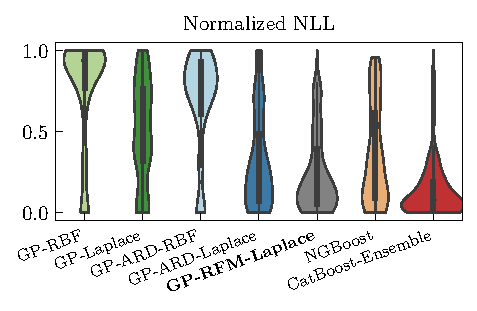
\includegraphics[trim=0 40 0 0, clip, width=\textwidth]{figures/tabularbenchmark_nll.pdf}
    \end{subfigure}
    % \hfill
    \begin{subfigure}[b]{0.475\textwidth}
        \centering
        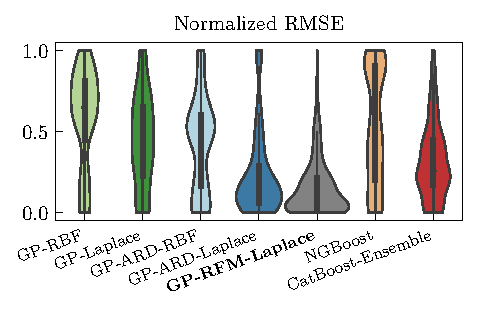
\includegraphics[trim=0 40 0 0, clip, width=\textwidth]{figures/tabularbenchmark_rmse.pdf}
    \end{subfigure}
    % \vskip\baselineskip
    \begin{subfigure}[b]{0.475\textwidth}
        \centering
        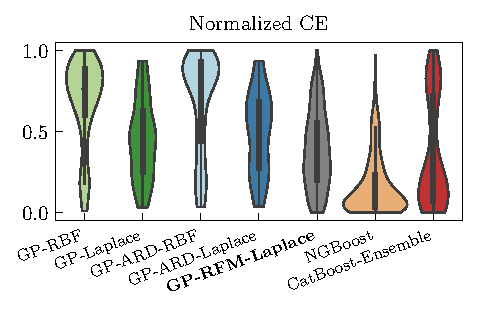
\includegraphics[width=\textwidth]{figures/tabularbenchmark_coverage.pdf}
    \end{subfigure}
    \caption{Violin plot results on OpenML benchmark datasets.}
    \label{fig:main-tabular-benchmark}
\end{figure}

% \daniel{plot of interval len rank vs coverage}








\subsection{Toy data set}
Given the qualitatively similar performance of the GP-RFM-Laplace and the GP-ARD-Laplace, we investigate the differences between the two methods in more detail.
Mathematically, the ARD kernel is equivalent to the RFM kernel with a diagonal feature matrix, learnt through NLL minimization instead of AGOP iterations.
Therefore, the RFM kernel can be seen as a generalization of the ARD kernel which can capture feature correlations which are relevant for the predictive task.

To highlight the difference between both kernels, we generate a toy dataset
where the features are independent $\vx\sim\gN(0,\mI_d)$ and the labels are the squared sum of the first 10 features $y=(\sum_{i=1}^{10} \vx_{[i]})^2$.
This dataset is designed to be challenging for the ARD kernel as it requires learning the feature correlation.
We compare the performance for a range of feature sizes in \Cref{fig:toy-data-nll}; the respective results for RMSE can be found in the appendix.

We observe that the GP-RFM-Laplace outperforms the GP-ARD-Laplace for all feature sizes.
Therefore, we conjecture that in the real-world datasets which we consider, there is either little feature correlation or the feature correlation is not relevant for the predictive task.
For datasets where the GP-RFM-Laplace considerably outperforms the GP-ARD-Laplace, such as the ISOLET (Isolated Letter Speech Recognition) dataset from OpenML, we observe that there is indeed considerable feature correlation.

\begin{figure}
    \centering
    % \includegraphics{figuresTikz/toy_data_nll}
    % \tikzsetnextfilename{toy_data_nll}
    \begin{tikzpicture}[baseline]

\pgfplotstableread[col sep=comma]{./data/toy_data_metrics.csv}{\datatable};
\begin{axis}[
width=\columnwidth,
height=.7\columnwidth,
ylabel={NLL},
xlabel={features $d$},
title={Toy data with feature correlation},
xmin=19,
xmax=131,
% ymin=0,
% ymax=0.5,
legend style={font=\tiny, 
	fill opacity=0.6, text opacity =1,
        at={(0.98,.18)},anchor=south east,
        row sep=-3pt,
        },
legend cell align={left},
% ytick={0, 0.08}, % Define the desired y tick positions
xtick={10, 30, 50, 70, 90, 110, 130}, % Define the desired y tick positions
yticklabel style={
	% /pgf/number format/fixed, % Use fixed point notation
	% /pgf/number format/precision=2, % Set the number of decimal places
	% /pgf/number format/fixed zerofill, % Fill in trailing zeros
        },
% ymode=log,
]


% RFM full
\addplot+ [black, 
mark=*,
mark options={solid},
% mark size=5pt,
thick,
error bars/.cd,
x dir=both,x explicit,
y dir=both,y explicit,
error bar style={solid}
]
table[x=features,y=GP_RFM_Laplace_full_NLPD_mean,y error=GP_RFM_Laplace_full_NLPD_std] {\datatable};

% % RFM diag
% \addplot+ [red, mark=x, mark size=5pt, thick,
% error bars/.cd,
% x dir=both,x explicit,
% y dir=both,y explicit,
% error bar style={solid}
% ]
% table[x=features,y=GP_RFM_Laplace_diag_NLPD_mean,y error=GP_RFM_Laplace_diag_NLPD_std] {\datatable};

% Laplace
\addplot+ [darkgreen, 
mark=*,
mark options={solid},
% mark size=5pt, 
thick,
error bars/.cd,
x dir=both,x explicit,
y dir=both,y explicit,
error bar style={solid}
]
table[x=features,y=GP_Laplace_NLPD_mean,y error=GP_Laplace_NLPD_std] {\datatable};

% ARD-Laplace
\addplot+ [darkblue, 
dotted,
mark=*,
mark options={solid},
% mark size=5pt, 
thick,
error bars/.cd,
x dir=both,x explicit,
y dir=both,y explicit,
error bar style={solid}
]
table[x=features,y=GP_ARD_Laplace_NLPD_mean,y error=GP_ARD_Laplace_NLPD_std] {\datatable};

% NG-boost
\addplot+ [orange,
dashed,
mark=*,
mark options={solid},
% mark size=5pt,
thick,
error bars/.cd,
x dir=both,x explicit,
y dir=both,y explicit,
error bar style={solid}
]
table[x=features,y=NG_Boost_NLPD_mean,y error=NG_Boost_NLPD_std] {\datatable};

% Cat-Boost Ensemble
\addplot+ [red, 
dashed,
mark=*,
mark options={solid},
% mark size=5pt, 
thick,
error bars/.cd,
x dir=both,x explicit,
y dir=both,y explicit,
error bar style={solid}
]
table[x=features,y=Cat_Boost_Ensemble_NLPD_mean,y error=Cat_Boost_Ensemble_NLPD_std] {\datatable};



\legend{
    {GP-RFM},
    {GP-Laplace}, 
    % {GP-RFM-diag},
    {GP-ARD-Laplace},
    {NGBoost},
    {CatBoost Ens.}
}

\end{axis}
\end{tikzpicture}
    \caption{Toy dataset with relevant feature correlation for prediction. We scale the number of train samples with $n=20 d$.}
    \label{fig:toy-data-nll}
\end{figure}








\subsection{Comparative feature evaluation}
Given the comparable performance of the GP-RFM-Laplace and the GP-ARD-Laplace, a second question arises regarding the learned features.
To investigate this, we compare the correlation between the diagonal of the feature matrix of the GP-RFM-Laplace and the GP-ARD-Laplace.
Additionally, we train a GP-RFM-Laplace where we restrict the feature matrix $\mM$ to be diagonal, i.e. we use the RFM-diag kernel.

\Cref{fig:feature-correlation} shows the correlation between the diagonal of the feature matrix for all three methods on the UCI benchmark datasets.
While there is a high correlation between all three methods for some datasets, there are also datasets where the correlation is low--even between the methods learning diagonal features, the RFM-diag and the GP-ARD-Laplace.
This indicates that learning the features with AGOP in the RFM or with NLL minimization in the ARD kernel
may result in the same features in some cases but is not guaranteed to do so.
Further investigation is required to understand the differences between feature learning in the two methods.


\begin{figure}
    \centering
    % \includegraphics{figuresTikz/feature_correlation}
    % \tikzsetnextfilename{feature_correlation}
    \begin{tikzpicture}
\pgfplotstableread[col sep=comma]{./data/correlation_rfmfull_rfmdiag.csv}{\datatableA};
\pgfplotstableread[col sep=comma]{./data/correlation_rfmfull_ard.csv}{\datatableB};
\pgfplotstableread[col sep=comma]{./data/correlation_rfmdiag_ard.csv}{\datatableC};
\begin{axis}[
boxplot/draw direction=y,
title={Feature correlation},
width=\columnwidth,
height=0.7\columnwidth,
boxplot={
	%
	% Idea: 
	%  place the 
	%  group 1 at 0.25 and 0.5 and 0.75
	%  group 2 at 1.25 and 1.5 and 1.75
	%  group 3 at 2.25 and 2.5 and 2.75
	%  ...
	% in a formular:
%	draw position={0.25 + floor(\plotnumofactualtype/3) + 0.25*mod(\plotnumofactualtype,3)},
	draw position={0.25 + floor(\plotnumofactualtype/3) + 0.25*mod(\plotnumofactualtype,3)},
	%
	% that means the box extend must be at most 0.2 :
	box extend=0.2,
},
% ... it also means that 1 unit in x controls the width:
%x=1.5cm,
xtick={0,1,2,...,8},
%xtick={0.5,1.5,2.5,3.5,4.5,5.5,6.5}
x tick label as interval,
xticklabels={%
	{YaHy},%
	{Ki},%
	{CoCoSt},%
	{CoCyPoPl},%
	{EnEf},%
	{NaPlMa},%
	{WiQuRe},%
},
xticklabel style={rotate=45, anchor=east}, % Rotate labels by 45 degrees
xmin=0,
xmax=7,
ymax=1.1,
ymin=-0.75,
legend style={font=\tiny, 
	fill opacity=0.9, text opacity=1,
	at={(0.02,0.02)},
	anchor=south west,
	row sep=0pt},
legend cell align={left},
area legend,
legend entries = {
	{RFM vs RFM-diag},
	{RFM vs ARD-Laplace},
	{RFM-diag vs ARD-Laplace},
},
]

%YaHy
\addplot[boxplot, thick, draw=darkblue] table[y index=6] {\datatableA};
\addplot[boxplot, thick, draw=darkgreen] table[y index=6] {\datatableC};
\addplot[boxplot, thick, draw=red] table[y index=6] {\datatableC};

%Ki
\addplot[boxplot, thick, draw=darkblue] table[y index=2] {\datatableA};
\addplot[boxplot, thick, draw=darkgreen] table[y index=2] {\datatableB};
\addplot[boxplot, thick, draw=red] table[y index=2] {\datatableC};

% CoCoSt
\addplot[boxplot, thick, draw=darkblue] table[y index=0] {\datatableA};
\addplot[boxplot, thick, draw=darkgreen] table[y index=0] {\datatableB};
\addplot[boxplot, thick, draw=red] table[y index=0] {\datatableC};

%CoCyPoPl
\addplot[boxplot, thick, draw=darkblue] table[y index=4] {\datatableA};
\addplot[boxplot, thick, draw=darkgreen] table[y index=4] {\datatableB};
\addplot[boxplot, thick, draw=red] table[y index=4] {\datatableC};

% EnEf
\addplot[boxplot, thick, draw=darkblue] table[y index=1] {\datatableA};
\addplot[boxplot, thick, draw=darkgreen] table[y index=1] {\datatableB};
\addplot[boxplot, thick, draw=red] table[y index=1] {\datatableC};

%NaPlMa
\addplot[boxplot, thick, draw=darkblue] table[y index=3] {\datatableA};
\addplot[boxplot, thick, draw=darkgreen] table[y index=3] {\datatableB};
\addplot[boxplot, thick, draw=red] table[y index=3] {\datatableC};

%WiQuRe
\addplot[boxplot, thick, draw=darkblue] table[y index=5] {\datatableA};
\addplot[boxplot, thick, draw=darkgreen] table[y index=5] {\datatableB};
\addplot[boxplot, thick, draw=red] table[y index=5] {\datatableC};


%\addplot[color=darkblue] plot coordinates {(4,15) (10,25)};
%\addplot[color=darkgreen] plot coordinates {(4,15) (10,25)};
%\addplot[color=red] plot coordinates {(4,15) (10,25)};

\end{axis}
\end{tikzpicture}
    \caption{Boxplot of correlation between the diagonal of weight matrix in RFM, RFM-diag and ARD-Laplace for all UCI benchmark datasets.
        \hl{Figure has an error that for WiQuRe the blue box is for some reason not in the right spot.}
        }
    \label{fig:feature-correlation}
\end{figure}





\subsection{Out-of-distribution data}
% motivation for OOD data
Having established that the GP-RFM-Laplace is a competitive method for probabilistic regression, we now investigate its performance on out-of-distribution (OOD) data.
Distribution shift depicts a common scenario in real-world applications where for example the test data distribution changes over time.
One hope of utilizing a probabilistic model is to obtain more reliable predictions by indicating when the model is uncertain about its predictions.
Understanding how well the GP-RFM-Laplace performs in such scenarios is essential for assessing its robustness and applicability in real-world settings.

% definition of OOD in our setting
In our setting, we concentrate on real-world data shifts.
Here, we focus on label shifts, i.e. the marginal distribution of the labels $p(y)$ change,
while in the appendix we also consider feature shifts, i.e. the marginal distribution of the features $p(\vx)$ change.
Specifically, we consider the Houses dataset from the OpenML benchmark where the labels are the median house value ranging in this dataset from 10.5 to 13.5.
For label shift, we define the in-distribution (ID) data as $p(y\geq11.75)$.
Then, we define different severities of label shift by considering $p(11.75>y\geq11.5)$, $p(11.5>y\geq11.25)$, $p(11.25>y\geq11)$ and $p(11>y)$.
This results in four OOD datasets with increasing severity of label shift.

% results and interpretation
\Cref{fig:ood-main_paper} shows the results for the NLL on ID and OOD data for different methods.
We notice that as expected the NLL of all methods rises with increasing severity of label shift.
However, the GP-RFM-Laplace is the most robust method, followed by the GP-ARD-Laplace.
This reliability is confirmed by the low CE of the GP-based methods which shows that the model is better calibrated under label shift which is shown in the appendix.
Boosting-based methods are less robust to label shifts from our scenario.


\begin{figure}
    \centering
    % \includegraphics{figuresTikz/ood_main_paper}
    % \tikzsetnextfilename{ood_main_paper}
    % and store the number of columns in `\NoOfCols'
% (minus 1 because counting in `\foreach' starts with zero
% \pgfplotstablegetcolsof{\loadedtable}
% \pgfmathtruncatemacro{\NoOfCols}{\pgfplotsretval-1}
% \NoOfCols

\begin{tikzpicture}[baseline]
    \pgfplotstableread[col sep=comma]{./data/ood_label_metrics.csv}{\loadedtable};
    
    \begin{axis}[
        % adjust the `width' a bit by keeping the default `height'
        width=\columnwidth,
        height=0.7\columnwidth,
        title={NLL on label shift},
        % ymin=1e-1,
        ymax=9,
        % there should be no gap between the bars in one group
        ybar=0pt,
        % adjust the size of the bars so they don't overlap
        bar width=0.85/5, % divided by number of columns
        % enlarge the x limits so all of the bars are shown
        enlarge x limits={abs=0.6},
        xtick={0, 1, 2, 3, 4}, % Define the desired y tick positions
        xticklabels={ID, OOD-1, OOD-2, OOD-3, OOD-4},
        legend style={font=\tiny, 
	fill opacity=0.6, text opacity =1,
        at={(0.02, 0.98)},anchor=north west,
        row sep=-3pt,
        },
        legend cell align={left},
    ]

        % GP-ARD-Laplace
        \addplot[fill=darkblue] table [
            x expr=\coordindex,
            y index=16, % zero based
            col sep=comma,
        ] {\loadedtable};

        % GP-RFM-Laplace
        \addplot[fill=black] table [
            x expr=\coordindex,
            y index=21,
            col sep=comma,
        ] {\loadedtable};

        % NGBoost
        \addplot[fill=orange] table [
            x expr=\coordindex,
            y index=26,
            col sep=comma,
        ] {\loadedtable};

        % CatBoost-Ensemble
        \addplot[fill=red] table [
            x expr=\coordindex,
            y index=31,
            col sep=comma,
        ] {\loadedtable};

        \legend{
            % {GP-RBF},
            % {GP-Laplace},
            % {GP-ARD-RBF},
            {GP-ARD-Laplace},
            {GP-RFM-Laplace}, 
            {NGBoost},
            {CatBoost-Ensemble}
        }
    \end{axis}
\end{tikzpicture}
    \caption{
        \hl{Title TODO}
        }
    \label{fig:ood-main_paper}
\end{figure}







\subsection{Neural networks as feature extractor}
\hl{TODO as experiment does not give any good results right now}

\csvreader[late after line=]{
		data/neural_network_metrics.csv
	}{
	% mean
		NN-Ensemble RMSE mean=\rmseA_, NN-Ensemble NLPD mean=\nlpdA_, NN-Ensemble Coverage mean=\covA_, NN-Ensemble Interval Len mean=\intA_,
		NN-RFM-EGOP RMSE mean=\rmseB_, NN-RFM-EGOP NLPD mean=\nlpdB_, NN-RFM-EGOP Coverage mean=\covB_, NN-RFM-EGOP Interval Len mean=\intB_,
		NN-RFM-NFA RMSE mean=\rmseC_, NN-RFM-NFA NLPD mean=\nlpdC_, NN-RFM-NFA Coverage mean=\covC_, NN-RFM-NFA Interval Len mean=\intC_,
		GP-RFM-Laplace RMSE mean=\rmseD_, GP-RFM-Laplace NLPD mean=\nlpdD_, GP-RFM-Laplace Coverage mean=\covD_, GP-RFM-Laplace Interval Len mean=\intD_,
	% std
		NN-Ensemble RMSE std=\rmseAstd_, NN-Ensemble NLPD std=\nlpdAstd_, NN-Ensemble Coverage std=\covAstd_, NN-Ensemble Interval Len std=\intAstd_,
		NN-RFM-EGOP RMSE std=\rmseBstd_, NN-RFM-EGOP NLPD std=\nlpdBstd_, NN-RFM-EGOP Coverage std=\covBstd_, NN-RFM-EGOP Interval Len std=\intBstd_,
		NN-RFM-NFA RMSE std=\rmseCstd_, NN-RFM-NFA NLPD std=\nlpdCstd_, NN-RFM-NFA Coverage std=\covCstd_, NN-RFM-NFA Interval Len std=\intCstd_,
            GP-RFM-Laplace RMSE std=\rmseDstd_, GP-RFM-Laplace NLPD std=\nlpdDstd_, GP-RFM-Laplace Coverage std=\covDstd_, GP-RFM-Laplace Interval Len std=\intDstd_,
	}{
		% mean
		\xdef\lastrmseA_{\rmseA_} \xdef\lastnlpdA_{\nlpdA_} \xdef\lastcovA_{\covA_} \xdef\lastintA_{\intA_}
		\xdef\lastrmseB_{\rmseB_} \xdef\lastnlpdB_{\nlpdB_} \xdef\lastcovB_{\covB_} \xdef\lastintB_{\intB_}
		\xdef\lastrmseC_{\rmseC_} \xdef\lastnlpdC_{\nlpdC_} \xdef\lastcovC_{\covC_} \xdef\lastintC_{\intC_}
		\xdef\lastrmseD_{\rmseD_} \xdef\lastnlpdD_{\nlpdD_} \xdef\lastcovD_{\covD_} \xdef\lastintD_{\intD_}
		% std
		\xdef\lastrmseAstd_{\rmseAstd_} \xdef\lastnlpdAstd_{\nlpdAstd_} \xdef\lastcovAstd_{\covAstd_} \xdef\lastintAstd_{\intAstd_}
		\xdef\lastrmseBstd_{\rmseBstd_} \xdef\lastnlpdBstd_{\nlpdBstd_} \xdef\lastcovBstd_{\covBstd_} \xdef\lastintBstd_{\intBstd_}
		\xdef\lastrmseCstd_{\rmseCstd_} \xdef\lastnlpdCstd_{\nlpdCstd_} \xdef\lastcovCstd_{\covCstd_} \xdef\lastintCstd_{\intCstd_}
		\xdef\lastrmseDstd_{\rmseDstd_} \xdef\lastnlpdDstd_{\nlpdDstd_} \xdef\lastcovDstd_{\covDstd_} \xdef\lastintDstd_{\intDstd_}
	}
\begin{table}[htb]
    \centering
    \caption{
        \hl{Title TODO}\\
        \daniel{explanation: comparison with NN-features on isolet dataset (613 features; RFM was best of basic methods). \\
        \textbf{NN Ensemble}: ensemble of 5 neural networks with ReLU FCN with feature sizes in the layers 613-256-64-16-1. \\
        \textbf{NN+RFM (NFA)}: one neural network where we take the input features to the last layers and replace the last layer with a GP-RFM-Laplace with a fixed feature matrix from the last layer of the NN. \\
        \textbf{NN+RFM}: one neural network where we take the pre-activation features of the 2nd to last layer and replace the last layer with a GP-RFM-Laplace learnt with EGOP. \\
        \textbf{RFM}: Baseline GP-RFM-Laplace directly from input features.\\
        We repeat over 20 seeds and report mean and std.}\\
        }
    % % \resizebox{\columnwidth}{!}{%
    % \begin{tabular}{l|llll}
    %     \toprule
    %         & RMSE ($\downarrow$) & NLL ($\downarrow$) & Cov. ($\downarrow$) & Interval ($\downarrow$) \\
    %     \midrule
    %     RFM          	& \lastrmseD_ \scriptsize{$\pm$\lastrmseDstd_} & \lastnlpdD_ \scriptsize{$\pm$\lastnlpdDstd_} & \lastcovD_ \scriptsize{$\pm$\lastcovDstd_} & \lastintD_ \scriptsize{$\pm$\lastintDstd_} \\
    %     NN Ensemble		& \lastrmseA_ \scriptsize{$\pm$\lastrmseAstd_} & \lastnlpdA_ \scriptsize{$\pm$\lastnlpdAstd_} & \lastcovA_ \scriptsize{$\pm$\lastcovAstd_} & \lastintA_ \scriptsize{$\pm$\lastintAstd_} \\
    %     NN+RFM (NFA)	& \lastrmseC_ \scriptsize{$\pm$\lastrmseCstd_} & \lastnlpdC_ \scriptsize{$\pm$\lastnlpdCstd_} & \lastcovC_ \scriptsize{$\pm$\lastcovCstd_} & \lastintC_ \scriptsize{$\pm$\lastintCstd_} \\
    %     NN+RFM & \lastrmseB_ \scriptsize{$\pm$\lastrmseBstd_} & \lastnlpdB_ \scriptsize{$\pm$\lastnlpdBstd_} & \lastcovB_ \scriptsize{$\pm$\lastcovBstd_} & \lastintB_ \scriptsize{$\pm$\lastintBstd_} \\
    %     \bottomrule
    % \end{tabular}
    % % }

    % \begin{tabular}{l|llll}
    %     \toprule
    %      & RFM & NN-Ens. & NN-RFM (NFA) & NN-RFM \\
    %     \midrule
    %     RMSE            & \lastrmseD_ \scriptsize{$\pm$\lastrmseDstd_}  & \lastrmseA_ \scriptsize{$\pm$\lastrmseAstd_}  & \lastrmseC_ \scriptsize{$\pm$\lastrmseCstd_}  & \lastrmseB_ \scriptsize{$\pm$\lastrmseBstd_}  \\
    %     NLL             & \lastnlpdD_ \scriptsize{$\pm$\lastnlpdDstd_}  & \lastnlpdA_ \scriptsize{$\pm$\lastnlpdAstd_}  & \lastnlpdC_ \scriptsize{$\pm$\lastnlpdCstd_}  & \lastnlpdB_ \scriptsize{$\pm$\lastnlpdBstd_}  \\
    %     Cov. Err.       & \lastcovD_ \scriptsize{$\pm$\lastcovDstd_}    & \lastcovA_ \scriptsize{$\pm$\lastcovAstd_}    & \lastcovC_ \scriptsize{$\pm$\lastcovCstd_}    & \lastcovB_ \scriptsize{$\pm$\lastcovBstd_}    \\
    %     Intval. Len.    & \lastintD_ \scriptsize{$\pm$\lastintDstd_}    & \lastintA_ \scriptsize{$\pm$\lastintAstd_}    & \lastintC_ \scriptsize{$\pm$\lastintCstd_}    & \lastintB_ \scriptsize{$\pm$\lastintBstd_}    \\
    %     \bottomrule
    % \end{tabular}

    \begin{tabular}{l|ll|ll}
        \toprule
         & RFM & NN-Ens. & \multicolumn{2}{c}{NN-RFM} \\
         &      & & NFA & AGOP \\
        \midrule
        % RMSE            & \lastrmseD_   & \lastrmseA_   & \lastrmseC_   & \lastrmseB_  \\
        % NLL             & \lastnlpdD_   & \lastnlpdA_   & \lastnlpdC_   & \lastnlpdB_  \\
        % Cov. Err.       & \lastcovD_    & \lastcovA_    & \lastcovC_    & \lastcovB_    \\
        % Intval. Len.    & \lastintD_    & \lastintA_    & \lastintC_    & \lastintB_    \\
        \bottomrule
    \end{tabular}

\end{table}







\subsection{Regularization and thresholding}
\hl{We don't have any experiments or ablations here}
\section{DISCUSSION}

\begin{itemize}
    \item Discussion between ARD and Diagonal-RFM
    \item neural networks and potential of our method to be incorporated with them.
\end{itemize}


\clearpage
\hrule\hrule
\hl{\textbf{Submissions are limited to 8 pages excluding references using the LaTeX style file we provide below (the page limit will be 9 for camera-ready submissions}).}
\hrule\hrule



\subsubsection*{Acknowledgements}
\hl{
All acknowledgments go at the end of the paper, including thanks to reviewers who gave useful comments, to colleagues who contributed to the ideas, and to funding agencies and corporate sponsors that provided financial support. 
To preserve the anonymity, please include acknowledgments \emph{only} in the camera-ready papers.
}\\
This work was partially supported by the Wallenberg AI, Autonomous Systems and Software Program (WASP) funded by the Knut and Alice Wallenberg Foundation. % DG
The computations were enabled by the Berzelius resource provided by the Knut and Alice Wallenberg Foundation at the National Supercomputer Centre, Sweden. % DG





% references
\bibliographystyle{apalike}
\bibliography{references}





\clearpage
%%%%%%%%%%%%%%%%%%%%%%%%%%%%%%%%%%%%%%%%%%%%%%%%%%%%%%%%%%%%
\section*{Checklist}


% %%% BEGIN INSTRUCTIONS %%%
The checklist follows the references. For each question, choose your answer from the three possible options: Yes, No, Not Applicable.  You are encouraged to include a justification to your answer, either by referencing the appropriate section of your paper or providing a brief inline description (1-2 sentences). 
Please do not modify the questions.  Note that the Checklist section does not count towards the page limit. Not including the checklist in the first submission won't result in desk rejection, although in such case we will ask you to upload it during the author response period and include it in camera ready (if accepted).

\textbf{In your paper, please delete this instructions block and only keep the Checklist section heading above along with the questions/answers below.}
% %%% END INSTRUCTIONS %%%


 \begin{enumerate}


 \item For all models and algorithms presented, check if you include:
 \begin{enumerate}
   \item A clear description of the mathematical setting, assumptions, algorithm, and/or model. [\hl{Yes}/No/Not Applicable]
   \item An analysis of the properties and complexity (time, space, sample size) of any algorithm. [Yes/\hl{No}/Not Applicable]
   \item (Optional) Anonymized source code, with specification of all dependencies, including external libraries. [Yes/\hl{No}/Not Applicable]
 \end{enumerate}


 \item For any theoretical claim, check if you include:
 \begin{enumerate}
   \item Statements of the full set of assumptions of all theoretical results. [Yes/No/Not Applicable]
   \item Complete proofs of all theoretical results. [Yes/No/Not Applicable]
   \item Clear explanations of any assumptions. [Yes/No/Not Applicable]     
 \end{enumerate}


 \item For all figures and tables that present empirical results, check if you include:
 \begin{enumerate}
   \item The code, data, and instructions needed to reproduce the main experimental results (either in the supplemental material or as a URL). [Yes/No/Not Applicable]
   \item All the training details (e.g., data splits, hyperparameters, how they were chosen). [Yes/No/Not Applicable]
         \item A clear definition of the specific measure or statistics and error bars (e.g., with respect to the random seed after running experiments multiple times). [Yes/No/Not Applicable]
         \item A description of the computing infrastructure used. (e.g., type of GPUs, internal cluster, or cloud provider). [Yes/No/Not Applicable]
 \end{enumerate}

 \item If you are using existing assets (e.g., code, data, models) or curating/releasing new assets, check if you include:
 \begin{enumerate}
   \item Citations of the creator If your work uses existing assets. [Yes/No/Not Applicable]
   \item The license information of the assets, if applicable. [Yes/No/Not Applicable]
   \item New assets either in the supplemental material or as a URL, if applicable. [Yes/No/Not Applicable]
   \item Information about consent from data providers/curators. [Yes/No/Not Applicable]
   \item Discussion of sensible content if applicable, e.g., personally identifiable information or offensive content. [Yes/No/Not Applicable]
 \end{enumerate}

 \item If you used crowdsourcing or conducted research with human subjects, check if you include:
 \begin{enumerate}
   \item The full text of instructions given to participants and screenshots. [Yes/No/Not Applicable]
   \item Descriptions of potential participant risks, with links to Institutional Review Board (IRB) approvals if applicable. [Yes/No/Not Applicable]
   \item The estimated hourly wage paid to participants and the total amount spent on participant compensation. [Yes/No/Not Applicable]
 \end{enumerate}

 \end{enumerate}







\clearpage
\appendix
\onecolumn
\daniel{we have to remove this later as AISTATS wants the supplementary to be a separate document}
\hrule
\begin{center}
    \textbf{\Large{Supplementary Materials}}
\end{center}
\hrule
\section{ADDITIONAL EXPERIMENTS}







\subsection{Main results}

\begin{figure*}[htb]
    \centering
    \begin{subfigure}[b]{0.475\textwidth}
        \centering
        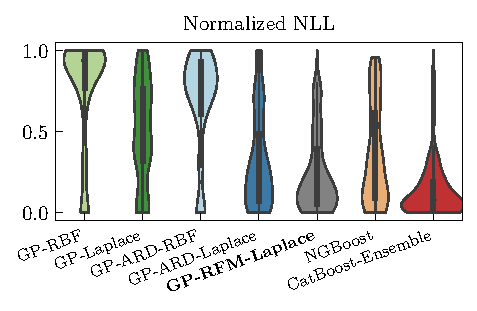
\includegraphics[trim=0 40 0 0, clip, width=\textwidth]{figures/tabularbenchmark_nll.pdf}
    \end{subfigure}
    \hfill
    \begin{subfigure}[b]{0.475\textwidth}  
        \centering 
        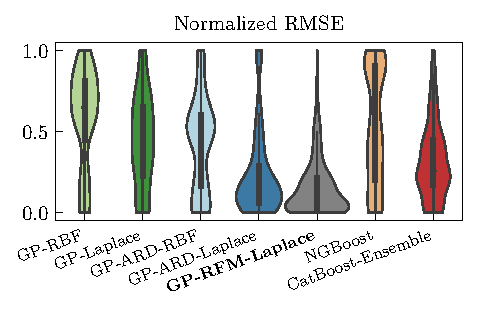
\includegraphics[trim=0 40 0 0, clip, width=\textwidth]{figures/tabularbenchmark_rmse.pdf}
    \end{subfigure}
    % \vskip\baselineskip
    \begin{subfigure}[b]{0.475\textwidth}   
        \centering 
        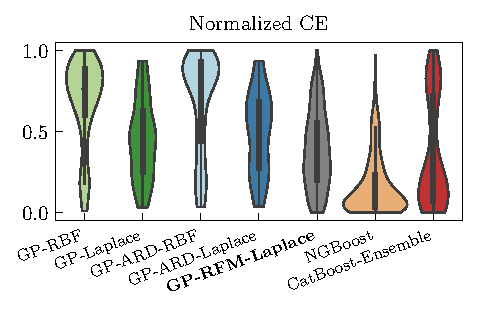
\includegraphics[width=\textwidth]{figures/tabularbenchmark_coverage.pdf}
    \end{subfigure}
    \hfill
    \begin{subfigure}[b]{0.475\textwidth}   
        \centering 
        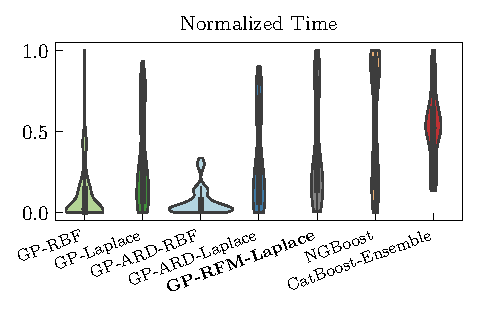
\includegraphics[width=\textwidth]{figures/tabularbenchmark_time.pdf}
    \end{subfigure}
    \caption{
        \hl{title TODO} results on tabular benchmark datasets
        \daniel{explanation: Every dataset of the 16 tabular benchmark dataset; tabular benchmark has more datasets/features/samples than uci benchmark we use; all hyperparameters are tuned; run everything for 20 seeds; for each dataset and metric we normalize the results of all methods in $[0,1]$; violin plot.}
        \daniel{use word 'coverage error'}
        } 
    \label{fig:main-tabular-benchmark-app}
\end{figure*}

\begin{figure*}[htb]
    \centering
    \begin{subfigure}[b]{0.475\textwidth}
        \centering
        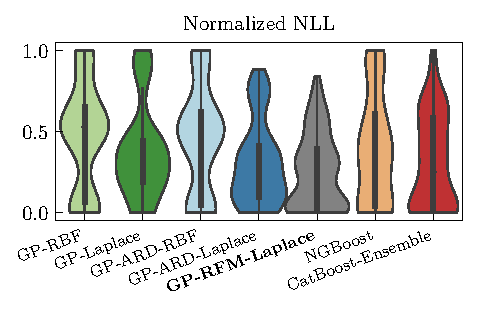
\includegraphics[trim=0 40 0 0, clip, width=\textwidth]{figures/uci_nll.pdf}
    \end{subfigure}
    \hfill
    \begin{subfigure}[b]{0.475\textwidth}  
        \centering 
        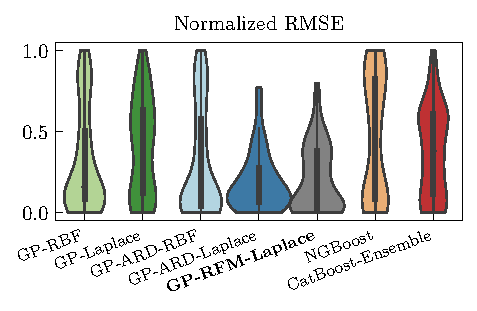
\includegraphics[trim=0 40 0 0, clip, width=\textwidth]{figures/uci_rmse.pdf}
    \end{subfigure}
    % \vskip\baselineskip
    \begin{subfigure}[b]{0.475\textwidth}   
        \centering 
        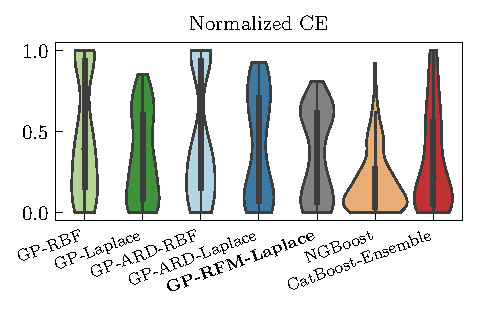
\includegraphics[width=\textwidth]{figures/uci_coverage.pdf}
    \end{subfigure}
    \hfill
    \begin{subfigure}[b]{0.475\textwidth}   
        \centering 
        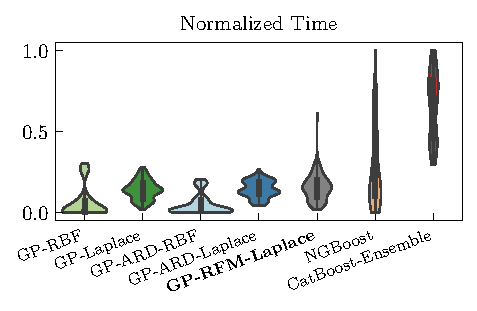
\includegraphics[width=\textwidth]{figures/uci_time.pdf}
    \end{subfigure}
    \caption{
        \hl{title TODO} results on UCI datasets. Complementary to \Cref{fig:main-tabular-benchmark}.
        \daniel{explanation: same as in \Cref{fig:main-tabular-benchmark}}
        } 
    \label{fig:main-uci}
\end{figure*}



\subsection{Comparative feature evaluation}



\begin{figure*}[htb]
    \centering
    \begin{subfigure}[b]{0.475\textwidth}
        \centering
        % \includegraphics{figuresTikz/feature_importance_nll}
        % \tikzsetnextfilename{feature_importance_nll}
        \begin{tikzpicture}[baseline]

\pgfplotstableread[col sep=comma]{./data/feature_importance_metrics.csv}{\datatable};
\begin{axis}[
width=\columnwidth,
height=.7\columnwidth,
ylabel={NLL},
xlabel={Fraction of remaining features},
title={Performance when removing features},
% ymax=0.3,
legend style={font=\tiny, 
	fill opacity=0.6, text opacity =1,
        at={(0.02, 0.02)},anchor=south west,
        row sep=-3pt,
        },
legend cell align={left},
% ytick={0, 0.08}, % Define the desired y tick positions
xtick={60, 70, 80, 90, 100}, % Define the desired y tick positions
xticklabels={60\%, 70\%, 80\%, 90\%, 100\%},
yticklabel style={
	% /pgf/number format/fixed, % Use fixed point notation
	% /pgf/number format/precision=2, % Set the number of decimal places
	% /pgf/number format/fixed zerofill, % Fill in trailing zeros
        },
% ymode=log,
]

% GP-RBF
\addplot+ [lightgreen, mark=*, 
mark options={solid},
thick,
% error bars/.cd,
% x dir=both,x explicit,
% y dir=both,y explicit,
% error bar style={solid}
]
table[x=features,y=GP_RBF_NLPD_mean,y error=GP_RBF_NLPD_std] {\datatable};


% GP-Laplace
\addplot+ [darkgreen, mark=*, 
mark options={solid},
thick,
% error bars/.cd,
% x dir=both,x explicit,
% y dir=both,y explicit,
% error bar style={solid}
]
table[x=features,y=GP_Laplace_NLPD_mean,y error=GP_Laplace_NLPD_std] {\datatable};


% GP-ARD-RBF
\addplot+ [lightblue, mark=*, 
mark options={solid},
thick,
dotted,
% error bars/.cd,
% x dir=both,x explicit,
% y dir=both,y explicit,
% error bar style={solid}
]
table[x=features,y=GP_ARD_RBF_NLPD_mean,y error=GP_ARD_RBF_NLPD_std] {\datatable};


% GP-ARD-Laplace
\addplot+ [darkblue, mark=*, 
mark options={solid},
thick,
dotted,
% error bars/.cd,
% x dir=both,x explicit,
% y dir=both,y explicit,
% error bar style={solid}
]
table[x=features,y=GP_ARD_Laplace_NLPD_mean,y error=GP_ARD_Laplace_NLPD_std] {\datatable};


% RFM
\addplot+ [black, mark=*, 
mark options={solid},
thick,
% error bars/.cd,
% x dir=both,x explicit,
% y dir=both,y explicit,
% error bar style={solid}
]
table[x=features,y=GP_RFM_Laplace_NLPD_mean,y error=GP_RFM_Laplace_NLPD_std] {\datatable};


% NG-Boost
\addplot+ [orange, mark=*, 
mark options={solid},
thick,
dashed,
% error bars/.cd,
% x dir=both,x explicit,
% y dir=both,y explicit,
% error bar style={solid}
]
table[x=features,y=NG_Boost_NLPD_mean,y error=GP_RFM_Laplace_NLPD_std] {\datatable};


% Cat-Boost-Ensemble
\addplot+ [red, mark=*, 
mark options={solid},
thick,
dashed,
% error bars/.cd,
% x dir=both,x explicit,
% y dir=both,y explicit,
% error bar style={solid}
]
table[x=features,y=Cat_Boost_Ensemble_NLPD_mean,y error=Cat_Boost_Ensemble_NLPD_std] {\datatable};



\legend{
    {GP-RBF},
    {GP-Laplace},
    {GP-ARD-RBF},
    {GP-ARD-Laplace},
    {GP-RFM-Laplace}, 
    {NGBoost},
    {CatBoost-Ensemble}
}

\end{axis}
\end{tikzpicture}
    \end{subfigure}
    \hfill
    \begin{subfigure}[b]{0.475\textwidth}  
        \centering
        % \includegraphics{figuresTikz/feature_importance_rmse}
        % \tikzsetnextfilename{feature_importance_rmse}
        \begin{tikzpicture}[baseline]

\pgfplotstableread[col sep=comma]{./data/feature_importance_metrics.csv}{\datatable};
\begin{axis}[
width=1\columnwidth,
height=.7\columnwidth,
ylabel={RMSE},
xlabel={Fraction of remaining features},
title={Performance when removing features},
% ymax=0.3,
legend style={font=\tiny, 
	fill opacity=0.6, text opacity =1,
        at={(0.02, 0.02)},anchor=south west,
        row sep=-3pt,
        },
legend cell align={left},
% ytick={0, 0.08}, % Define the desired y tick positions
xtick={60, 70, 80, 90, 100}, % Define the desired y tick positions
xticklabels={60\%, 70\%, 80\%, 90\%, 100\%},
yticklabel style={
	% /pgf/number format/fixed, % Use fixed point notation
	% /pgf/number format/precision=2, % Set the number of decimal places
	% /pgf/number format/fixed zerofill, % Fill in trailing zeros
        },
% ymode=log,
]

% GP-RBF
\addplot+ [lightgreen, mark=*, 
mark options={solid},
thick,
% error bars/.cd,
% x dir=both,x explicit,
% y dir=both,y explicit,
% error bar style={solid}
]
table[x=features,y=GP_RBF_RMSE_mean,y error=GP_RBF_RMSE_std] {\datatable};


% GP-Laplace
\addplot+ [darkgreen, mark=*, 
mark options={solid},
thick,
% error bars/.cd,
% x dir=both,x explicit,
% y dir=both,y explicit,
% error bar style={solid}
]
table[x=features,y=GP_Laplace_RMSE_mean,y error=GP_Laplace_RMSE_std] {\datatable};


% GP-ARD-RBF
\addplot+ [lightblue, mark=*, 
mark options={solid},
thick,
dotted,
% error bars/.cd,
% x dir=both,x explicit,
% y dir=both,y explicit,
% error bar style={solid}
]
table[x=features,y=GP_ARD_RBF_RMSE_mean,y error=GP_ARD_RBF_RMSE_std] {\datatable};


% GP-ARD-Laplace
\addplot+ [darkblue, mark=*, 
mark options={solid},
thick,
dotted,
% error bars/.cd,
% x dir=both,x explicit,
% y dir=both,y explicit,
% error bar style={solid}
]
table[x=features,y=GP_ARD_Laplace_RMSE_mean,y error=GP_ARD_Laplace_RMSE_std] {\datatable};


% RFM
\addplot+ [black, mark=*, 
mark options={solid},
thick,
% error bars/.cd,
% x dir=both,x explicit,
% y dir=both,y explicit,
% error bar style={solid}
]
table[x=features,y=GP_RFM_Laplace_RMSE_mean,y error=GP_RFM_Laplace_RMSE_std] {\datatable};


% NG-Boost
\addplot+ [orange, mark=*, 
mark options={solid},
thick,
dashed,
% error bars/.cd,
% x dir=both,x explicit,
% y dir=both,y explicit,
% error bar style={solid}
]
table[x=features,y=NG_Boost_RMSE_mean,y error=GP_RFM_Laplace_RMSE_std] {\datatable};


% Cat-Boost-Ensemble
\addplot+ [red, mark=*, 
mark options={solid},
thick,
dashed,
% error bars/.cd,
% x dir=both,x explicit,
% y dir=both,y explicit,
% error bar style={solid}
]
table[x=features,y=Cat_Boost_Ensemble_RMSE_mean,y error=Cat_Boost_Ensemble_RMSE_std] {\datatable};



\legend{
    {GP-RBF},
    {GP-Laplace},
    {GP-ARD-RBF},
    {GP-ARD-Laplace},
    {GP-RFM-Laplace}, 
    {NGBoost},
    {CatBoost Ensemble}
}

\end{axis}
\end{tikzpicture}
    \end{subfigure}
    \caption{NLL (left) and RMSE (right) when removing the most important features according to the diagonal of the RFM weight matrix.} 
    \label{fig:feature-importance}
\end{figure*}
    







\subsection{Toy data set}

\begin{figure}[htb]
    \centering
    % \includegraphics{figuresTikz/toy_data_rmse}
    % \tikzsetnextfilename{toy_data_rmse}
    \begin{tikzpicture}[baseline]

\pgfplotstableread[col sep=comma]{./data/toy_data_metrics.csv}{\datatable};
\begin{axis}[
width=0.5\columnwidth,
height=.35\columnwidth,
ylabel={RMSE},
xlabel={features},
title={Toy data with feature correlation},
xmin=19,
xmax=131,
% ymin=0,
% ymax=0.33,
legend style={font=\tiny, 
	fill opacity=0.6, text opacity =1,
        % at={(1.,1)},anchor=north east,
        row sep=-3pt,
        },
legend cell align={left},
% ytick={0, 0.08}, % Define the desired y tick positions
xtick={10, 30, 50, 70, 90, 110, 130}, % Define the desired y tick positions
yticklabel style={
	% /pgf/number format/fixed, % Use fixed point notation
	% /pgf/number format/precision=2, % Set the number of decimal places
	% /pgf/number format/fixed zerofill, % Fill in trailing zeros
        },
% ymode=log,
]


% RFM full
\addplot+ [black, 
mark=*, 
mark options={solid},
% mark size=5pt, 
thick,
error bars/.cd,
x dir=both,x explicit,
y dir=both,y explicit,
error bar style={solid}
]
table[x=features,y=GP_RFM_Laplace_full_RMSE_mean,y error=GP_RFM_Laplace_full_RMSE_std] {\datatable};

% % RFM diag
% \addplot+ [red, mark=x, mark size=5pt, thick,
% error bars/.cd,
% x dir=both,x explicit,
% y dir=both,y explicit,
% error bar style={solid}
% ]
% table[x=features,y=GP_RFM_Laplace_diag_RMSE_mean,y error=GP_RFM_Laplace_diag_RMSE_std] {\datatable};

% Laplace
\addplot+ [darkgreen, 
mark=*, 
mark options={solid},
% mark size=5pt, 
thick,
error bars/.cd,
x dir=both,x explicit,
y dir=both,y explicit,
error bar style={solid}
]
table[x=features,y=GP_Laplace_RMSE_mean,y error=GP_Laplace_RMSE_std] {\datatable};

% ARD-Laplace
\addplot+ [darkblue, 
dotted,
mark=*, 
mark options={solid},
% mark size=5pt, 
thick,
error bars/.cd,
x dir=both,x explicit,
y dir=both,y explicit,
error bar style={solid}
]
table[x=features,y=GP_ARD_Laplace_RMSE_mean,y error=GP_ARD_Laplace_RMSE_std] {\datatable};

% NG-boost
\addplot+ [orange, 
dashed,
mark=*, 
mark options={solid},
% mark size=5pt, 
thick,
error bars/.cd,
x dir=both,x explicit,
y dir=both,y explicit,
error bar style={solid}
]
table[x=features,y=NG_Boost_RMSE_mean,y error=NG_Boost_RMSE_std] {\datatable};

% Cat-Boost Ensemble
\addplot+ [red, 
dashed,
mark=*, 
mark options={solid},
% mark size=5pt, 
thick,
error bars/.cd,
x dir=both,x explicit,
y dir=both,y explicit,
error bar style={solid}
]
table[x=features,y=Cat_Boost_Ensemble_RMSE_mean,y error=Cat_Boost_Ensemble_RMSE_std] {\datatable};



\legend{
    {GP-RFM}, 
    {GP-Laplace},
    % {GP-RFM-diag},
    {GP-ARD-Laplace},
    {NGBoost},
    {CatBoost Ensemble}
}

\end{axis}
\end{tikzpicture}
    \caption{
        \hl{Title TODO} Complementary to \Cref{fig:toy-data-nll} but showing RMSE instead of NLL here.
        \daniel{Explanation: Same as in \Cref{fig:toy-data-nll}.}
        }
    \label{fig:toy-data-rmse}
\end{figure}

\hl{Include figure about learnt feature matrix in RFM, RFM-diag and ARD-Laplace as comprison}








\subsection{Distribution shift}


\begin{figure*}[htb]
    \centering
    \begin{subfigure}[b]{0.475\textwidth}
        \centering
        % \includegraphics{figuresTikz/ood_covariate_nll}
        % \tikzsetnextfilename{ood_covariate_nll}
        \begin{tikzpicture}[baseline]

\pgfplotstableread[col sep=comma]{./data/ood_covariate_metrics.csv}{\datatable};
\begin{axis}[
width=\columnwidth,
height=.7\columnwidth,
% ylabel={NLL},
% xlabel={},
title={NLL},
ymax=2,
legend style={font=\tiny, 
	fill opacity=0.6, text opacity =1,
        at={(0.02, 0.98)},anchor=north west,
        row sep=-3pt,
        },
legend cell align={left},
% ytick={0, 0.08}, % Define the desired y tick positions
xtick={0, 1,2,3,4}, % Define the desired y tick positions
xticklabels={ID, OOD-1, OOD-2, OOD-3, OOD-4},
yticklabel style={
	% /pgf/number format/fixed, % Use fixed point notation
	% /pgf/number format/precision=2, % Set the number of decimal places
	% /pgf/number format/fixed zerofill, % Fill in trailing zeros
        },
% ymode=log,
]

% GP-RBF
\addplot+ [lightgreen, mark=*, 
mark options={solid},
thick,
% error bars/.cd,
% x dir=both,x explicit,
% y dir=both,y explicit,
% error bar style={solid}
]
table[x=test_level,y=GP_RBF_NLPD_mean,y error=GP_RBF_NLPD_std] {\datatable};


% GP-Laplace
\addplot+ [darkgreen, mark=*, 
mark options={solid},
thick,
% error bars/.cd,
% x dir=both,x explicit,
% y dir=both,y explicit,
% error bar style={solid}
]
table[x=test_level,y=GP_Laplace_NLPD_mean,y error=GP_Laplace_NLPD_std] {\datatable};


% GP-ARD-RBF
\addplot+ [lightblue, mark=*, 
mark options={solid},
thick,
dotted,
% error bars/.cd,
% x dir=both,x explicit,
% y dir=both,y explicit,
% error bar style={solid}
]
table[x=test_level,y=GP_ARD_RBF_NLPD_mean,y error=GP_ARD_RBF_NLPD_std] {\datatable};


% GP-ARD-Laplace
\addplot+ [darkblue, mark=*, 
mark options={solid},
thick,
dotted,
% error bars/.cd,
% x dir=both,x explicit,
% y dir=both,y explicit,
% error bar style={solid}
]
table[x=test_level,y=GP_ARD_Laplace_NLPD_mean,y error=GP_ARD_Laplace_NLPD_std] {\datatable};


% RFM
\addplot+ [black, mark=*, 
mark options={solid},
thick,
% error bars/.cd,
% x dir=both,x explicit,
% y dir=both,y explicit,
% error bar style={solid}
]
table[x=test_level,y=GP_RFM_Laplace_NLPD_mean,y error=GP_RFM_Laplace_NLPD_std] {\datatable};


% NG-Boost
\addplot+ [orange, mark=*, 
mark options={solid},
thick,
dashed,
% error bars/.cd,
% x dir=both,x explicit,
% y dir=both,y explicit,
% error bar style={solid}
]
table[x=test_level,y=NG_Boost_NLPD_mean,y error=GP_RFM_Laplace_NLPD_std] {\datatable};


% Cat-Boost-Ensemble
\addplot+ [red, mark=*, 
mark options={solid},
thick,
dashed,
% error bars/.cd,
% x dir=both,x explicit,
% y dir=both,y explicit,
% error bar style={solid}
]
table[x=test_level,y=Cat_Boost_Ensemble_NLPD_mean,y error=Cat_Boost_Ensemble_NLPD_std] {\datatable};



% \legend{
%     {GP-RBF},
%     {GP-Laplace},
%     {GP-ARD-RBF},
%     {GP-ARD-Laplace},
%     {GP-RFM-Laplace}, 
%     {NGBoost},
%     {CatBoost-Ensemble}
% }

\end{axis}
\end{tikzpicture}
    \end{subfigure}
    \hfill
    \begin{subfigure}[b]{0.475\textwidth}  
        \centering
        % \includegraphics{figuresTikz/ood_covariate_rmse}
        % \tikzsetnextfilename{ood_covariate_rmse}
        \begin{tikzpicture}[baseline]

\pgfplotstableread[col sep=comma]{./data/ood_covariate_metrics.csv}{\datatable};
\begin{axis}[
width=\columnwidth,
height=.7\columnwidth,
% ylabel={RMSE},
% xlabel={},
title={RMSE},
% ymax=2,
legend style={font=\tiny, 
	fill opacity=0.6, text opacity =1,
        at={(0.02, 0.98)},anchor=north west,
        row sep=-3pt,
        },
legend cell align={left},
% ytick={0, 0.08}, % Define the desired y tick positions
xtick={0, 1,2,3,4}, % Define the desired y tick positions
xticklabels={ID, OOD-1, OOD-2, OOD-3, OOD-4},
yticklabel style={
	% /pgf/number format/fixed, % Use fixed point notation
	% /pgf/number format/precision=2, % Set the number of decimal places
	% /pgf/number format/fixed zerofill, % Fill in trailing zeros
        },
% ymode=log,
]

% GP-RBF
\addplot+ [lightgreen, mark=*, 
mark options={solid},
thick,
% error bars/.cd,
% x dir=both,x explicit,
% y dir=both,y explicit,
% error bar style={solid}
]
table[x=test_level,y=GP_RBF_RMSE_mean,y error=GP_RBF_RMSE_std] {\datatable};


% GP-Laplace
\addplot+ [darkgreen, mark=*, 
mark options={solid},
thick,
% error bars/.cd,
% x dir=both,x explicit,
% y dir=both,y explicit,
% error bar style={solid}
]
table[x=test_level,y=GP_Laplace_RMSE_mean,y error=GP_Laplace_RMSE_std] {\datatable};


% GP-ARD-RBF
\addplot+ [lightblue, mark=*, 
mark options={solid},
thick,
dotted,
% error bars/.cd,
% x dir=both,x explicit,
% y dir=both,y explicit,
% error bar style={solid}
]
table[x=test_level,y=GP_ARD_RBF_RMSE_mean,y error=GP_ARD_RBF_RMSE_std] {\datatable};


% GP-ARD-Laplace
\addplot+ [darkblue, mark=*, 
mark options={solid},
thick,
dotted,
% error bars/.cd,
% x dir=both,x explicit,
% y dir=both,y explicit,
% error bar style={solid}
]
table[x=test_level,y=GP_ARD_Laplace_RMSE_mean,y error=GP_ARD_Laplace_RMSE_std] {\datatable};


% RFM
\addplot+ [black, mark=*, 
mark options={solid},
thick,
% error bars/.cd,
% x dir=both,x explicit,
% y dir=both,y explicit,
% error bar style={solid}
]
table[x=test_level,y=GP_RFM_Laplace_RMSE_mean,y error=GP_RFM_Laplace_RMSE_std] {\datatable};


% NG-Boost
\addplot+ [orange, mark=*, 
mark options={solid},
thick,
dashed,
% error bars/.cd,
% x dir=both,x explicit,
% y dir=both,y explicit,
% error bar style={solid}
]
table[x=test_level,y=NG_Boost_RMSE_mean,y error=GP_RFM_Laplace_RMSE_std] {\datatable};


% Cat-Boost-Ensemble
\addplot+ [red, mark=*, 
mark options={solid},
thick,
dashed,
% error bars/.cd,
% x dir=both,x explicit,
% y dir=both,y explicit,
% error bar style={solid}
]
table[x=test_level,y=Cat_Boost_Ensemble_RMSE_mean,y error=Cat_Boost_Ensemble_RMSE_std] {\datatable};



\legend{
    {GP-RBF},
    {GP-Laplace},
    {GP-ARD-RBF},
    {GP-ARD-Laplace},
    {GP-RFM-Laplace}, 
    {NGBoost},
    {CatBoost-Ensemble}
}

\end{axis}
\end{tikzpicture}
    \end{subfigure}
    % \vskip\baselineskip
    \begin{subfigure}[b]{0.475\textwidth}   
        \centering
        % \includegraphics{figuresTikz/ood_covariate_coverage}
        % \tikzsetnextfilename{ood_covariate_coverage}
        \begin{tikzpicture}[baseline]

\pgfplotstableread[col sep=comma]{./data/ood_covariate_metrics.csv}{\datatable};
\begin{axis}[
width=\columnwidth,
height=.7\columnwidth,
% ylabel={Coverage},
% xlabel={},
title={Coverage Error},
% ymax=2,
legend style={font=\tiny, 
	fill opacity=0.6, text opacity =1,
        at={(0.02, 0.98)},anchor=north west,
        row sep=-3pt,
        },
legend cell align={left},
% ytick={0, 0.08}, % Define the desired y tick positions
xtick={0, 1,2,3,4}, % Define the desired y tick positions
xticklabels={ID, OOD-1, OOD-2, OOD-3, OOD-4},
yticklabel style={
	% /pgf/number format/fixed, % Use fixed point notation
	% /pgf/number format/precision=2, % Set the number of decimal places
	% /pgf/number format/fixed zerofill, % Fill in trailing zeros
        },
% ymode=log,
]

% GP-RBF
\addplot+ [lightgreen, mark=*, 
mark options={solid},
thick,
% error bars/.cd,
% x dir=both,x explicit,
% y dir=both,y explicit,
% error bar style={solid}
]
table[x=test_level,y=GP_RBF_Coverage_mean,y error=GP_RBF_Coverage_std] {\datatable};


% GP-Laplace
\addplot+ [darkgreen, mark=*, 
mark options={solid},
thick,
% error bars/.cd,
% x dir=both,x explicit,
% y dir=both,y explicit,
% error bar style={solid}
]
table[x=test_level,y=GP_Laplace_Coverage_mean,y error=GP_Laplace_Coverage_std] {\datatable};


% GP-ARD-RBF
\addplot+ [lightblue, mark=*, 
mark options={solid},
thick,
dotted,
% error bars/.cd,
% x dir=both,x explicit,
% y dir=both,y explicit,
% error bar style={solid}
]
table[x=test_level,y=GP_ARD_RBF_Coverage_mean,y error=GP_ARD_RBF_Coverage_std] {\datatable};


% GP-ARD-Laplace
\addplot+ [darkblue, mark=*, 
mark options={solid},
thick,
dotted,
% error bars/.cd,
% x dir=both,x explicit,
% y dir=both,y explicit,
% error bar style={solid}
]
table[x=test_level,y=GP_ARD_Laplace_Coverage_mean,y error=GP_ARD_Laplace_Coverage_std] {\datatable};


% RFM
\addplot+ [black, mark=*, 
mark options={solid},
thick,
% error bars/.cd,
% x dir=both,x explicit,
% y dir=both,y explicit,
% error bar style={solid}
]
table[x=test_level,y=GP_RFM_Laplace_Coverage_mean,y error=GP_RFM_Laplace_Coverage_std] {\datatable};


% NG-Boost
\addplot+ [orange, mark=*, 
mark options={solid},
thick,
dashed,
% error bars/.cd,
% x dir=both,x explicit,
% y dir=both,y explicit,
% error bar style={solid}
]
table[x=test_level,y=NG_Boost_Coverage_mean,y error=GP_RFM_Laplace_Coverage_std] {\datatable};


% Cat-Boost-Ensemble
\addplot+ [red, mark=*, 
mark options={solid},
thick,
dashed,
% error bars/.cd,
% x dir=both,x explicit,
% y dir=both,y explicit,
% error bar style={solid}
]
table[x=test_level,y=Cat_Boost_Ensemble_Coverage_mean,y error=Cat_Boost_Ensemble_Coverage_std] {\datatable};



% \legend{
%     {GP-RBF},
%     {GP-Laplace},
%     {GP-ARD-RBF},
%     {GP-ARD-Laplace},
%     {GP-RFM-Laplace}, 
%     {NGBoost},
%     {CatBoost-Ensemble}
% }

\end{axis}
\end{tikzpicture}
    \end{subfigure}     
    \hfill
    \begin{subfigure}[b]{0.475\textwidth}   
        \centering 
        % \includegraphics{figuresTikz/ood_covariate_intvallen}
        % \tikzsetnextfilename{ood_covariate_intvallen}
        \begin{tikzpicture}[baseline]

\pgfplotstableread[col sep=comma]{./data/ood_covariate_metrics.csv}{\datatable};
\begin{axis}[
width=\columnwidth,
height=.7\columnwidth,
% ylabel={Interval_Len},
% xlabel={},
title={Interval Length},
% ymax=2,
legend style={font=\tiny, 
	fill opacity=0.6, text opacity =1,
        at={(0.02, 0.98)},anchor=north west,
        row sep=-3pt,
        },
legend cell align={left},
% ytick={0, 0.08}, % Define the desired y tick positions
xtick={0, 1,2,3,4}, % Define the desired y tick positions
xticklabels={ID, OOD-1, OOD-2, OOD-3, OOD-4},
yticklabel style={
	% /pgf/number format/fixed, % Use fixed point notation
	% /pgf/number format/precision=2, % Set the number of decimal places
	% /pgf/number format/fixed zerofill, % Fill in trailing zeros
        },
% ymode=log,
]

% GP-RBF
\addplot+ [lightgreen, mark=*, 
mark options={solid},
thick,
% error bars/.cd,
% x dir=both,x explicit,
% y dir=both,y explicit,
% error bar style={solid}
]
table[x=test_level,y=GP_RBF_Interval_Len_mean,y error=GP_RBF_Interval_Len_std] {\datatable};


% GP-Laplace
\addplot+ [darkgreen, mark=*, 
mark options={solid},
thick,
% error bars/.cd,
% x dir=both,x explicit,
% y dir=both,y explicit,
% error bar style={solid}
]
table[x=test_level,y=GP_Laplace_Interval_Len_mean,y error=GP_Laplace_Interval_Len_std] {\datatable};


% GP-ARD-RBF
\addplot+ [lightblue, mark=*, 
mark options={solid},
thick,
dotted,
% error bars/.cd,
% x dir=both,x explicit,
% y dir=both,y explicit,
% error bar style={solid}
]
table[x=test_level,y=GP_ARD_RBF_Interval_Len_mean,y error=GP_ARD_RBF_Interval_Len_std] {\datatable};


% GP-ARD-Laplace
\addplot+ [darkblue, mark=*, 
mark options={solid},
thick,
dotted,
% error bars/.cd,
% x dir=both,x explicit,
% y dir=both,y explicit,
% error bar style={solid}
]
table[x=test_level,y=GP_ARD_Laplace_Interval_Len_mean,y error=GP_ARD_Laplace_Interval_Len_std] {\datatable};


% RFM
\addplot+ [black, mark=*, 
mark options={solid},
thick,
% error bars/.cd,
% x dir=both,x explicit,
% y dir=both,y explicit,
% error bar style={solid}
]
table[x=test_level,y=GP_RFM_Laplace_Interval_Len_mean,y error=GP_RFM_Laplace_Interval_Len_std] {\datatable};


% NG-Boost
\addplot+ [orange, mark=*, 
mark options={solid},
thick,
dashed,
% error bars/.cd,
% x dir=both,x explicit,
% y dir=both,y explicit,
% error bar style={solid}
]
table[x=test_level,y=NG_Boost_Interval_Len_mean,y error=GP_RFM_Laplace_Interval_Len_std] {\datatable};


% Cat-Boost-Ensemble
\addplot+ [red, mark=*, 
mark options={solid},
thick,
dashed,
% error bars/.cd,
% x dir=both,x explicit,
% y dir=both,y explicit,
% error bar style={solid}
]
table[x=test_level,y=Cat_Boost_Ensemble_Interval_Len_mean,y error=Cat_Boost_Ensemble_Interval_Len_std] {\datatable};



% \legend{
%     {GP-RBF},
%     {GP-Laplace},
%     {GP-ARD-RBF},
%     {GP-ARD-Laplace},
%     {GP-RFM-Laplace}, 
%     {NGBoost},
%     {CatBoost-Ensemble}
% }

\end{axis}
\end{tikzpicture}
    \end{subfigure}
    \caption{
        \hl{title TODO} Covariate shift......
        } 
    \label{fig:ood-covariate-appendix}
\end{figure*}


\begin{figure*}[htb]
    \centering
    \begin{subfigure}[b]{0.475\textwidth}
        \centering
        % \includegraphics{figuresTikz/ood_label_nll}
        % \tikzsetnextfilename{ood_label_nll}
        \begin{tikzpicture}[baseline]

\pgfplotstableread[col sep=comma]{./data/ood_label_metrics.csv}{\datatable};
\begin{axis}[
width=\columnwidth,
height=.7\columnwidth,
% ylabel={NLL},
% xlabel={},
title={NLL},
ymax=9,
legend style={font=\tiny, 
	fill opacity=0.6, text opacity =1,
        at={(0.02, 0.98)},anchor=north west,
        row sep=-3pt,
        },
legend cell align={left},
% ytick={0, 0.08}, % Define the desired y tick positions
xtick={0, 1,2,3,4}, % Define the desired y tick positions
xticklabels={ID, OOD-1, OOD-2, OOD-3, OOD-4},
yticklabel style={
	% /pgf/number format/fixed, % Use fixed point notation
	% /pgf/number format/precision=2, % Set the number of decimal places
	% /pgf/number format/fixed zerofill, % Fill in trailing zeros
        },
% ymode=log,
]

% GP-RBF
\addplot+ [lightgreen, mark=*, 
mark options={solid},
thick,
% error bars/.cd,
% x dir=both,x explicit,
% y dir=both,y explicit,
% error bar style={solid}
]
table[x=test_level,y=GP_RBF_NLPD_mean,y error=GP_RBF_NLPD_std] {\datatable};


% GP-Laplace
\addplot+ [darkgreen, mark=*, 
mark options={solid},
thick,
% error bars/.cd,
% x dir=both,x explicit,
% y dir=both,y explicit,
% error bar style={solid}
]
table[x=test_level,y=GP_Laplace_NLPD_mean,y error=GP_Laplace_NLPD_std] {\datatable};


% GP-ARD-RBF
\addplot+ [lightblue, mark=*, 
mark options={solid},
thick,
dotted,
% error bars/.cd,
% x dir=both,x explicit,
% y dir=both,y explicit,
% error bar style={solid}
]
table[x=test_level,y=GP_ARD_RBF_NLPD_mean,y error=GP_ARD_RBF_NLPD_std] {\datatable};


% GP-ARD-Laplace
\addplot+ [darkblue, mark=*, 
mark options={solid},
thick,
dotted,
% error bars/.cd,
% x dir=both,x explicit,
% y dir=both,y explicit,
% error bar style={solid}
]
table[x=test_level,y=GP_ARD_Laplace_NLPD_mean,y error=GP_ARD_Laplace_NLPD_std] {\datatable};


% RFM
\addplot+ [black, mark=*, 
mark options={solid},
thick,
% error bars/.cd,
% x dir=both,x explicit,
% y dir=both,y explicit,
% error bar style={solid}
]
table[x=test_level,y=GP_RFM_Laplace_NLPD_mean,y error=GP_RFM_Laplace_NLPD_std] {\datatable};


% NG-Boost
\addplot+ [orange, mark=*, 
mark options={solid},
thick,
dashed,
% error bars/.cd,
% x dir=both,x explicit,
% y dir=both,y explicit,
% error bar style={solid}
]
table[x=test_level,y=NG_Boost_NLPD_mean,y error=GP_RFM_Laplace_NLPD_std] {\datatable};


% Cat-Boost-Ensemble
\addplot+ [red, mark=*, 
mark options={solid},
thick,
dashed,
% error bars/.cd,
% x dir=both,x explicit,
% y dir=both,y explicit,
% error bar style={solid}
]
table[x=test_level,y=Cat_Boost_Ensemble_NLPD_mean,y error=Cat_Boost_Ensemble_NLPD_std] {\datatable};



% \legend{
%     {GP-RBF},
%     {GP-Laplace},
%     {GP-ARD-RBF},
%     {GP-ARD-Laplace},
%     {GP-RFM-Laplace}, 
%     {NGBoost},
%     {CatBoost-Ensemble}
% }

\end{axis}
\end{tikzpicture}
    \end{subfigure}
    \hfill
    \begin{subfigure}[b]{0.475\textwidth}  
        \centering
        % \includegraphics{figuresTikz/ood_label_rmse}
        % \tikzsetnextfilename{ood_label_rmse}
        \begin{tikzpicture}[baseline]

\pgfplotstableread[col sep=comma]{./data/ood_label_metrics.csv}{\datatable};
\begin{axis}[
width=\columnwidth,
height=.7\columnwidth,
% ylabel={RMSE},
% xlabel={},
title={RMSE},
% ymax=2,
legend style={font=\tiny, 
	fill opacity=0.6, text opacity =1,
        at={(0.02, 0.98)},anchor=north west,
        row sep=-3pt,
        },
legend cell align={left},
% ytick={0, 0.08}, % Define the desired y tick positions
xtick={0, 1,2,3,4}, % Define the desired y tick positions
xticklabels={ID, OOD-1, OOD-2, OOD-3, OOD-4},
yticklabel style={
	% /pgf/number format/fixed, % Use fixed point notation
	% /pgf/number format/precision=2, % Set the number of decimal places
	% /pgf/number format/fixed zerofill, % Fill in trailing zeros
        },
% ymode=log,
]

% GP-RBF
\addplot+ [lightgreen, mark=*, 
mark options={solid},
thick,
% error bars/.cd,
% x dir=both,x explicit,
% y dir=both,y explicit,
% error bar style={solid}
]
table[x=test_level,y=GP_RBF_RMSE_mean,y error=GP_RBF_RMSE_std] {\datatable};


% GP-Laplace
\addplot+ [darkgreen, mark=*, 
mark options={solid},
thick,
% error bars/.cd,
% x dir=both,x explicit,
% y dir=both,y explicit,
% error bar style={solid}
]
table[x=test_level,y=GP_Laplace_RMSE_mean,y error=GP_Laplace_RMSE_std] {\datatable};


% GP-ARD-RBF
\addplot+ [lightblue, mark=*, 
mark options={solid},
thick,
dotted,
% error bars/.cd,
% x dir=both,x explicit,
% y dir=both,y explicit,
% error bar style={solid}
]
table[x=test_level,y=GP_ARD_RBF_RMSE_mean,y error=GP_ARD_RBF_RMSE_std] {\datatable};


% GP-ARD-Laplace
\addplot+ [darkblue, mark=*, 
mark options={solid},
thick,
dotted,
% error bars/.cd,
% x dir=both,x explicit,
% y dir=both,y explicit,
% error bar style={solid}
]
table[x=test_level,y=GP_ARD_Laplace_RMSE_mean,y error=GP_ARD_Laplace_RMSE_std] {\datatable};


% RFM
\addplot+ [black, mark=*, 
mark options={solid},
thick,
% error bars/.cd,
% x dir=both,x explicit,
% y dir=both,y explicit,
% error bar style={solid}
]
table[x=test_level,y=GP_RFM_Laplace_RMSE_mean,y error=GP_RFM_Laplace_RMSE_std] {\datatable};


% NG-Boost
\addplot+ [orange, mark=*, 
mark options={solid},
thick,
dashed,
% error bars/.cd,
% x dir=both,x explicit,
% y dir=both,y explicit,
% error bar style={solid}
]
table[x=test_level,y=NG_Boost_RMSE_mean,y error=GP_RFM_Laplace_RMSE_std] {\datatable};


% Cat-Boost-Ensemble
\addplot+ [red, mark=*, 
mark options={solid},
thick,
dashed,
% error bars/.cd,
% x dir=both,x explicit,
% y dir=both,y explicit,
% error bar style={solid}
]
table[x=test_level,y=Cat_Boost_Ensemble_RMSE_mean,y error=Cat_Boost_Ensemble_RMSE_std] {\datatable};



\legend{
    {GP-RBF},
    {GP-Laplace},
    {GP-ARD-RBF},
    {GP-ARD-Laplace},
    {GP-RFM-Laplace}, 
    {NGBoost},
    {CatBoost-Ensemble}
}

\end{axis}
\end{tikzpicture}
    \end{subfigure}
    % \vskip\baselineskip
    \begin{subfigure}[b]{0.475\textwidth}   
        \centering
        % \includegraphics{figuresTikz/ood_label_coverage}
        % \tikzsetnextfilename{ood_label_coverage}
        \begin{tikzpicture}[baseline]

\pgfplotstableread[col sep=comma]{./data/ood_label_metrics.csv}{\datatable};
\begin{axis}[
width=\columnwidth,
height=.7\columnwidth,
% ylabel={Coverage},
% xlabel={},
title={Coverage Error},
% ymax=2,
legend style={font=\tiny, 
	fill opacity=0.6, text opacity =1,
        at={(0.02, 0.98)},anchor=north west,
        row sep=-3pt,
        },
legend cell align={left},
% ytick={0, 0.08}, % Define the desired y tick positions
xtick={0, 1,2,3,4}, % Define the desired y tick positions
xticklabels={ID, OOD-1, OOD-2, OOD-3, OOD-4},
yticklabel style={
	% /pgf/number format/fixed, % Use fixed point notation
	% /pgf/number format/precision=2, % Set the number of decimal places
	% /pgf/number format/fixed zerofill, % Fill in trailing zeros
        },
% ymode=log,
]

% GP-RBF
\addplot+ [lightgreen, mark=*, 
mark options={solid},
thick,
% error bars/.cd,
% x dir=both,x explicit,
% y dir=both,y explicit,
% error bar style={solid}
]
table[x=test_level,y=GP_RBF_Coverage_mean,y error=GP_RBF_Coverage_std] {\datatable};


% GP-Laplace
\addplot+ [darkgreen, mark=*, 
mark options={solid},
thick,
% error bars/.cd,
% x dir=both,x explicit,
% y dir=both,y explicit,
% error bar style={solid}
]
table[x=test_level,y=GP_Laplace_Coverage_mean,y error=GP_Laplace_Coverage_std] {\datatable};


% GP-ARD-RBF
\addplot+ [lightblue, mark=*, 
mark options={solid},
thick,
dotted,
% error bars/.cd,
% x dir=both,x explicit,
% y dir=both,y explicit,
% error bar style={solid}
]
table[x=test_level,y=GP_ARD_RBF_Coverage_mean,y error=GP_ARD_RBF_Coverage_std] {\datatable};


% GP-ARD-Laplace
\addplot+ [darkblue, mark=*, 
mark options={solid},
thick,
dotted,
% error bars/.cd,
% x dir=both,x explicit,
% y dir=both,y explicit,
% error bar style={solid}
]
table[x=test_level,y=GP_ARD_Laplace_Coverage_mean,y error=GP_ARD_Laplace_Coverage_std] {\datatable};


% RFM
\addplot+ [black, mark=*, 
mark options={solid},
thick,
% error bars/.cd,
% x dir=both,x explicit,
% y dir=both,y explicit,
% error bar style={solid}
]
table[x=test_level,y=GP_RFM_Laplace_Coverage_mean,y error=GP_RFM_Laplace_Coverage_std] {\datatable};


% NG-Boost
\addplot+ [orange, mark=*, 
mark options={solid},
thick,
dashed,
% error bars/.cd,
% x dir=both,x explicit,
% y dir=both,y explicit,
% error bar style={solid}
]
table[x=test_level,y=NG_Boost_Coverage_mean,y error=GP_RFM_Laplace_Coverage_std] {\datatable};


% Cat-Boost-Ensemble
\addplot+ [red, mark=*, 
mark options={solid},
thick,
dashed,
% error bars/.cd,
% x dir=both,x explicit,
% y dir=both,y explicit,
% error bar style={solid}
]
table[x=test_level,y=Cat_Boost_Ensemble_Coverage_mean,y error=Cat_Boost_Ensemble_Coverage_std] {\datatable};



% \legend{
%     {GP-RBF},
%     {GP-Laplace},
%     {GP-ARD-RBF},
%     {GP-ARD-Laplace},
%     {GP-RFM-Laplace}, 
%     {NGBoost},
%     {CatBoost-Ensemble}
% }

\end{axis}
\end{tikzpicture}
    \end{subfigure}
    \hfill
    \begin{subfigure}[b]{0.475\textwidth}   
        \centering 
        % \includegraphics{figuresTikz/ood_label_intvallen}
        % \tikzsetnextfilename{ood_label_intvallen}
        \begin{tikzpicture}[baseline]

\pgfplotstableread[col sep=comma]{./data/ood_label_metrics.csv}{\datatable};
\begin{axis}[
width=\columnwidth,
height=.7\columnwidth,
% ylabel={Interval_Len},
% xlabel={},
title={Interval Length},
% ymax=2,
legend style={font=\tiny, 
	fill opacity=0.6, text opacity =1,
        at={(0.02, 0.98)},anchor=north west,
        row sep=-3pt,
        },
legend cell align={left},
% ytick={0, 0.08}, % Define the desired y tick positions
xtick={0, 1,2,3,4}, % Define the desired y tick positions
xticklabels={ID, OOD-1, OOD-2, OOD-3, OOD-4},
yticklabel style={
	% /pgf/number format/fixed, % Use fixed point notation
	% /pgf/number format/precision=2, % Set the number of decimal places
	% /pgf/number format/fixed zerofill, % Fill in trailing zeros
        },
% ymode=log,
]

% GP-RBF
\addplot+ [lightgreen, mark=*, 
mark options={solid},
thick,
% error bars/.cd,
% x dir=both,x explicit,
% y dir=both,y explicit,
% error bar style={solid}
]
table[x=test_level,y=GP_RBF_Interval_Len_mean,y error=GP_RBF_Interval_Len_std] {\datatable};


% GP-Laplace
\addplot+ [darkgreen, mark=*, 
mark options={solid},
thick,
% error bars/.cd,
% x dir=both,x explicit,
% y dir=both,y explicit,
% error bar style={solid}
]
table[x=test_level,y=GP_Laplace_Interval_Len_mean,y error=GP_Laplace_Interval_Len_std] {\datatable};


% GP-ARD-RBF
\addplot+ [lightblue, mark=*, 
mark options={solid},
thick,
dotted,
% error bars/.cd,
% x dir=both,x explicit,
% y dir=both,y explicit,
% error bar style={solid}
]
table[x=test_level,y=GP_ARD_RBF_Interval_Len_mean,y error=GP_ARD_RBF_Interval_Len_std] {\datatable};


% GP-ARD-Laplace
\addplot+ [darkblue, mark=*, 
mark options={solid},
thick,
dotted,
% error bars/.cd,
% x dir=both,x explicit,
% y dir=both,y explicit,
% error bar style={solid}
]
table[x=test_level,y=GP_ARD_Laplace_Interval_Len_mean,y error=GP_ARD_Laplace_Interval_Len_std] {\datatable};


% RFM
\addplot+ [black, mark=*, 
mark options={solid},
thick,
% error bars/.cd,
% x dir=both,x explicit,
% y dir=both,y explicit,
% error bar style={solid}
]
table[x=test_level,y=GP_RFM_Laplace_Interval_Len_mean,y error=GP_RFM_Laplace_Interval_Len_std] {\datatable};


% NG-Boost
\addplot+ [orange, mark=*, 
mark options={solid},
thick,
dashed,
% error bars/.cd,
% x dir=both,x explicit,
% y dir=both,y explicit,
% error bar style={solid}
]
table[x=test_level,y=NG_Boost_Interval_Len_mean,y error=GP_RFM_Laplace_Interval_Len_std] {\datatable};


% Cat-Boost-Ensemble
\addplot+ [red, mark=*, 
mark options={solid},
thick,
dashed,
% error bars/.cd,
% x dir=both,x explicit,
% y dir=both,y explicit,
% error bar style={solid}
]
table[x=test_level,y=Cat_Boost_Ensemble_Interval_Len_mean,y error=Cat_Boost_Ensemble_Interval_Len_std] {\datatable};



% \legend{
%     {GP-RBF},
%     {GP-Laplace},
%     {GP-ARD-RBF},
%     {GP-ARD-Laplace},
%     {GP-RFM-Laplace}, 
%     {NGBoost},
%     {CatBoost-Ensemble}
% }

\end{axis}
\end{tikzpicture}
    \end{subfigure}
    \caption{
        \hl{title TODO} Label shift......
        } 
    \label{fig:ood-label-appendix}
\end{figure*}










\clearpage
\section{DETAILED RESULTS ON TABULAR BENCHMARKS}

\subsection{Tabular Benchmark}
% get the number of rows in table
\pgfplotstableread[col sep=comma]{data/tabularbenchmark/tabularbenchmark_results.csv}{\tabletabularbenchmark}
\pgfplotstablegetrowsof{\tabletabularbenchmark}
\pgfmathtruncatemacro{\NoOfRows}{\pgfplotsretval+1}
% for each dataset
\newcommand{\datalinktabularbenchmark}{data/tabularbenchmark/tabularbenchmark_results.csv}
\newcounter{datasetcounterOne}
\forloop{datasetcounterOne}{1}{\value{datasetcounterOne} < \NoOfRows}{
	\setcounter{rowcount}{0}
	\csvreader[late after line=]{
		\datalinktabularbenchmark
	}{
	% mean
		dataset=\dataset, samples=\samples, features=\features,
		GP-RBF RMSE=\rmseA_, GP-RBF NLPD=\nllA_, GP-RBF Coverage=\covA_, GP-RBF Interval Len=\intA_, GP-RBF Time=\timeA_, 
		GP-Laplace RMSE=\rmseB_, GP-Laplace NLPD=\nllB_, GP-Laplace Coverage=\covB_, GP-Laplace Interval Len=\intB_, GP-Laplace Time=\timeB_, 
		GP-ARD-RBF RMSE=\rmseC_, GP-ARD-RBF NLPD=\nllC_, GP-ARD-RBF Coverage=\covC_, GP-ARD-RBF Interval Len=\intC_, GP-ARD-RBF Time=\timeC_, 
		GP-ARD-Laplace RMSE=\rmseD_, GP-ARD-Laplace NLPD=\nllD_, GP-ARD-Laplace Coverage=\covD_, GP-ARD-Laplace Interval Len=\intD_,GP-ARD-Laplace Time=\timeD_, 
		GP-RFM-Laplace RMSE=\rmseE_, GP-RFM-Laplace NLPD=\nllE_, GP-RFM-Laplace Coverage=\covE_, GP-RFM-Laplace Interval Len=\intE_, GP-RFM-Laplace Time=\timeE_, 
		NG-Boost RMSE=\rmseF_, NG-Boost NLPD=\nllF_, NG-Boost Coverage=\covF_, NG-Boost Interval Len=\intF_, NG-Boost Time=\timeF_, 
		Cat-Boost-Ensemble RMSE=\rmseG_, Cat-Boost-Ensemble NLPD=\nllG_, Cat-Boost-Ensemble Coverage=\covG_, Cat-Boost-Ensemble Interval Len=\intG_, Cat-Boost-Ensemble Time=\timeG_, 
	% std
		GP-RBF RMSE std=\rmseAstd_, GP-RBF NLPD std=\nllAstd_, GP-RBF Coverage std=\covAstd_, GP-RBF Interval Len std=\intAstd_,GP-RBF Time std=\timeAstd_, 
		GP-Laplace RMSE std=\rmseBstd_, GP-Laplace NLPD std=\nllBstd_, GP-Laplace Coverage std=\covBstd_, GP-Laplace Interval Len std=\intBstd_, GP-Laplace Time std=\timeBstd_, 
		GP-ARD-RBF RMSE std=\rmseCstd_, GP-ARD-RBF NLPD std=\nllCstd_, GP-ARD-RBF Coverage std=\covCstd_, GP-ARD-RBF Interval Len std=\intCstd_, GP-ARD-RBF Time std=\timeCstd_, 
		GP-ARD-Laplace RMSE std=\rmseDstd_, GP-ARD-Laplace NLPD std=\nllDstd_, GP-ARD-Laplace Coverage std=\covDstd_, GP-ARD-Laplace Interval Len std=\intDstd_, GP-ARD-Laplace Time std=\timeDstd_, 
		GP-RFM-Laplace RMSE std=\rmseEstd_, GP-RFM-Laplace NLPD std=\nllEstd_, GP-RFM-Laplace Coverage std=\covEstd_, GP-RFM-Laplace Interval Len std=\intEstd_, GP-RFM-Laplace Time std=\timeEstd_, 
		NG-Boost RMSE std=\rmseFstd_, NG-Boost NLPD std=\nllFstd_, NG-Boost Coverage std=\covFstd_, NG-Boost Interval Len std=\intFstd_, NG-Boost Time std=\timeFstd_, 
		Cat-Boost-Ensemble RMSE std=\rmseGstd_, Cat-Boost-Ensemble NLPD std=\nllGstd_, Cat-Boost-Ensemble Coverage std=\covGstd_, Cat-Boost-Ensemble Interval Len std=\intGstd_, Cat-Boost-Ensemble Time std=\timeGstd_, 
	}{
		\stepcounter{rowcount}
		\ifnum\value{rowcount}=\thedatasetcounterOne% <-- Modify this line to specify the desired row number
		\xdef\lastdataset{\dataset} \xdef\lastsamples{\samples} \xdef\lastfeatures{\features} 
		% mean
		\xdef\lastrmseA_{\rmseA_} \xdef\lastnllA_{\nllA_} \xdef\lastcovA_{\covA_} \xdef\lastintA_{\intA_} \xdef\lasttimeA_{\timeA_}
		\xdef\lastrmseB_{\rmseB_} \xdef\lastnllB_{\nllB_} \xdef\lastcovB_{\covB_} \xdef\lastintB_{\intB_} \xdef\lasttimeB_{\timeB_}
		\xdef\lastrmseC_{\rmseC_} \xdef\lastnllC_{\nllC_} \xdef\lastcovC_{\covC_} \xdef\lastintC_{\intC_} \xdef\lasttimeC_{\timeC_}
		\xdef\lastrmseD_{\rmseD_} \xdef\lastnllD_{\nllD_} \xdef\lastcovD_{\covD_} \xdef\lastintD_{\intD_} \xdef\lasttimeD_{\timeD_}
		\xdef\lastrmseE_{\rmseE_} \xdef\lastnllE_{\nllE_} \xdef\lastcovE_{\covE_} \xdef\lastintE_{\intE_} \xdef\lasttimeE_{\timeE_}
		\xdef\lastrmseF_{\rmseF_} \xdef\lastnllF_{\nllF_} \xdef\lastcovF_{\covF_} \xdef\lastintF_{\intF_} \xdef\lasttimeF_{\timeF_}
		\xdef\lastrmseG_{\rmseG_} \xdef\lastnllG_{\nllG_} \xdef\lastcovG_{\covG_} \xdef\lastintG_{\intG_} \xdef\lasttimeG_{\timeG_}
		% std
		\xdef\lastrmseAstd_{\rmseAstd_} \xdef\lastnllAstd_{\nllAstd_} \xdef\lastcovAstd_{\covAstd_} \xdef\lastintAstd_{\intAstd_} \xdef\lasttimeAstd_{\timeAstd_}
		\xdef\lastrmseBstd_{\rmseBstd_} \xdef\lastnllBstd_{\nllBstd_} \xdef\lastcovBstd_{\covBstd_} \xdef\lastintBstd_{\intBstd_} \xdef\lasttimeBstd_{\timeBstd_}
		\xdef\lastrmseCstd_{\rmseCstd_} \xdef\lastnllCstd_{\nllCstd_} \xdef\lastcovCstd_{\covCstd_} \xdef\lastintCstd_{\intCstd_} \xdef\lasttimeCstd_{\timeCstd_}
		\xdef\lastrmseDstd_{\rmseDstd_} \xdef\lastnllDstd_{\nllDstd_} \xdef\lastcovDstd_{\covDstd_} \xdef\lastintDstd_{\intDstd_} \xdef\lasttimeDstd_{\timeDstd_}
		\xdef\lastrmseEstd_{\rmseEstd_} \xdef\lastnllEstd_{\nllEstd_} \xdef\lastcovEstd_{\covEstd_} \xdef\lastintEstd_{\intEstd_} \xdef\lasttimeEstd_{\timeEstd_}
		\xdef\lastrmseFstd_{\rmseFstd_} \xdef\lastnllFstd_{\nllFstd_} \xdef\lastcovFstd_{\covFstd_} \xdef\lastintFstd_{\intFstd_} \xdef\lasttimeFstd_{\timeFstd_}
		\xdef\lastrmseGstd_{\rmseGstd_} \xdef\lastnllGstd_{\nllGstd_} \xdef\lastcovGstd_{\covGstd_} \xdef\lastintGstd_{\intGstd_} \xdef\lasttimeGstd_{\timeGstd_}
		\fi
	}
	\begin{table}[htb]
		\centering
		\caption{Dataset: \lastdataset~(\lastsamples~samples; \lastfeatures~features)}
		% \resizebox{\textwidth}{!}{%
		\begin{tabular}{l||ll|ll|l}
			\toprule
			& RMSE ($\downarrow$) & NLL ($\downarrow$) & Cov. Err. ($\downarrow$) & Intval. ($\downarrow$) & Time ($\downarrow$) \\
			\midrule
			GP-RBF 			& \lastrmseA_ \scriptsize{$\pm$\lastrmseAstd_} & \lastnllA_ \scriptsize{$\pm$\lastnllAstd_} & \lastcovA_ \scriptsize{$\pm$\lastcovAstd_} & \lastintA_ \scriptsize{$\pm$\lastintAstd_} & \lasttimeA_ \scriptsize{$\pm$\lasttimeAstd_} \\
			GP-Laplace 		& \lastrmseB_ \scriptsize{$\pm$\lastrmseBstd_} & \lastnllB_ \scriptsize{$\pm$\lastnllBstd_} & \lastcovB_ \scriptsize{$\pm$\lastcovBstd_} & \lastintB_ \scriptsize{$\pm$\lastintBstd_} & \lasttimeB_ \scriptsize{$\pm$\lasttimeBstd_} \\
			\midrule
			GP-ARD-RBF 		& \lastrmseC_ \scriptsize{$\pm$\lastrmseCstd_} & \lastnllC_ \scriptsize{$\pm$\lastnllCstd_} & \lastcovC_ \scriptsize{$\pm$\lastcovCstd_} & \lastintC_ \scriptsize{$\pm$\lastintCstd_} & \lasttimeC_ \scriptsize{$\pm$\lasttimeCstd_} \\
			GP-ARD-Laplace 	& \lastrmseD_ \scriptsize{$\pm$\lastrmseDstd_} & \lastnllD_ \scriptsize{$\pm$\lastnllDstd_} & \lastcovD_ \scriptsize{$\pm$\lastcovDstd_} & \lastintD_ \scriptsize{$\pm$\lastintDstd_} & \lasttimeD_ \scriptsize{$\pm$\lasttimeDstd_} \\
			\midrule
			\textbf{GP-RFM-Laplace} 	& \lastrmseE_ \scriptsize{$\pm$\lastrmseEstd_} & \lastnllE_ \scriptsize{$\pm$\lastnllEstd_} & \lastcovE_ \scriptsize{$\pm$\lastcovEstd_} & \lastintE_ \scriptsize{$\pm$\lastintEstd_} & \lasttimeE_ \scriptsize{$\pm$\lasttimeEstd_} \\
			\midrule
			NGBoost 		& \lastrmseF_ \scriptsize{$\pm$\lastrmseFstd_} & \lastnllF_ \scriptsize{$\pm$\lastnllFstd_} & \lastcovF_ \scriptsize{$\pm$\lastcovFstd_} & \lastintF_ \scriptsize{$\pm$\lastintFstd_} & \lasttimeF_ \scriptsize{$\pm$\lasttimeFstd_} \\
			CatBoost-Ensemble 	& \lastrmseG_ \scriptsize{$\pm$\lastrmseGstd_} & \lastnllG_ \scriptsize{$\pm$\lastnllGstd_} & \lastcovG_ \scriptsize{$\pm$\lastcovGstd_} & \lastintG_ \scriptsize{$\pm$\lastintGstd_} & \lasttimeG_ \scriptsize{$\pm$\lasttimeGstd_} \\
			\bottomrule
		\end{tabular}
		% }
	\end{table}
}
\clearpage









\subsection{UCI benchmark}


% get the number of rows in table
\pgfplotstableread[col sep=comma]{data/uci/uci_results.csv}{\tableuci}
\pgfplotstablegetrowsof{\tableuci}
\pgfmathtruncatemacro{\NoOfRows}{\pgfplotsretval+1}
% for each dataset
\newcommand{\datalinkuci}{data/uci/uci_results.csv}
% \newcounter{datasetcounterOne}
\forloop{datasetcounterOne}{1}{\value{datasetcounterOne} < \NoOfRows}{
	\setcounter{rowcount}{0}
	\csvreader[late after line=]{
		\datalinkuci
	}{
	% mean
		dataset=\dataset, samples=\samples, features=\features,
		GP-RBF RMSE=\rmseA_, GP-RBF NLPD=\nllA_, GP-RBF Coverage=\covA_, GP-RBF Interval Len=\intA_, GP-RBF Time=\timeA_, 
		GP-Laplace RMSE=\rmseB_, GP-Laplace NLPD=\nllB_, GP-Laplace Coverage=\covB_, GP-Laplace Interval Len=\intB_, GP-Laplace Time=\timeB_, 
		GP-ARD-RBF RMSE=\rmseC_, GP-ARD-RBF NLPD=\nllC_, GP-ARD-RBF Coverage=\covC_, GP-ARD-RBF Interval Len=\intC_, GP-ARD-RBF Time=\timeC_, 
		GP-ARD-Laplace RMSE=\rmseD_, GP-ARD-Laplace NLPD=\nllD_, GP-ARD-Laplace Coverage=\covD_, GP-ARD-Laplace Interval Len=\intD_,GP-ARD-Laplace Time=\timeD_, 
		GP-RFM-Laplace RMSE=\rmseE_, GP-RFM-Laplace NLPD=\nllE_, GP-RFM-Laplace Coverage=\covE_, GP-RFM-Laplace Interval Len=\intE_, GP-RFM-Laplace Time=\timeE_, 
		NG-Boost RMSE=\rmseF_, NG-Boost NLPD=\nllF_, NG-Boost Coverage=\covF_, NG-Boost Interval Len=\intF_, NG-Boost Time=\timeF_, 
		Cat-Boost-Ensemble RMSE=\rmseG_, Cat-Boost-Ensemble NLPD=\nllG_, Cat-Boost-Ensemble Coverage=\covG_, Cat-Boost-Ensemble Interval Len=\intG_, Cat-Boost-Ensemble Time=\timeG_, 
	% std
		GP-RBF RMSE std=\rmseAstd_, GP-RBF NLPD std=\nllAstd_, GP-RBF Coverage std=\covAstd_, GP-RBF Interval Len std=\intAstd_,GP-RBF Time std=\timeAstd_, 
		GP-Laplace RMSE std=\rmseBstd_, GP-Laplace NLPD std=\nllBstd_, GP-Laplace Coverage std=\covBstd_, GP-Laplace Interval Len std=\intBstd_, GP-Laplace Time std=\timeBstd_, 
		GP-ARD-RBF RMSE std=\rmseCstd_, GP-ARD-RBF NLPD std=\nllCstd_, GP-ARD-RBF Coverage std=\covCstd_, GP-ARD-RBF Interval Len std=\intCstd_, GP-ARD-RBF Time std=\timeCstd_, 
		GP-ARD-Laplace RMSE std=\rmseDstd_, GP-ARD-Laplace NLPD std=\nllDstd_, GP-ARD-Laplace Coverage std=\covDstd_, GP-ARD-Laplace Interval Len std=\intDstd_, GP-ARD-Laplace Time std=\timeDstd_, 
		GP-RFM-Laplace RMSE std=\rmseEstd_, GP-RFM-Laplace NLPD std=\nllEstd_, GP-RFM-Laplace Coverage std=\covEstd_, GP-RFM-Laplace Interval Len std=\intEstd_, GP-RFM-Laplace Time std=\timeEstd_, 
		NG-Boost RMSE std=\rmseFstd_, NG-Boost NLPD std=\nllFstd_, NG-Boost Coverage std=\covFstd_, NG-Boost Interval Len std=\intFstd_, NG-Boost Time std=\timeFstd_, 
		Cat-Boost-Ensemble RMSE std=\rmseGstd_, Cat-Boost-Ensemble NLPD std=\nllGstd_, Cat-Boost-Ensemble Coverage std=\covGstd_, Cat-Boost-Ensemble Interval Len std=\intGstd_, Cat-Boost-Ensemble Time std=\timeGstd_, 
	}{
		\stepcounter{rowcount}
		\ifnum\value{rowcount}=\thedatasetcounterOne% <-- Modify this line to specify the desired row number
		\xdef\lastdataset{\dataset} \xdef\lastsamples{\samples} \xdef\lastfeatures{\features} 
		% mean
		\xdef\lastrmseA_{\rmseA_} \xdef\lastnllA_{\nllA_} \xdef\lastcovA_{\covA_} \xdef\lastintA_{\intA_} \xdef\lasttimeA_{\timeA_}
		\xdef\lastrmseB_{\rmseB_} \xdef\lastnllB_{\nllB_} \xdef\lastcovB_{\covB_} \xdef\lastintB_{\intB_} \xdef\lasttimeB_{\timeB_}
		\xdef\lastrmseC_{\rmseC_} \xdef\lastnllC_{\nllC_} \xdef\lastcovC_{\covC_} \xdef\lastintC_{\intC_} \xdef\lasttimeC_{\timeC_}
		\xdef\lastrmseD_{\rmseD_} \xdef\lastnllD_{\nllD_} \xdef\lastcovD_{\covD_} \xdef\lastintD_{\intD_} \xdef\lasttimeD_{\timeD_}
		\xdef\lastrmseE_{\rmseE_} \xdef\lastnllE_{\nllE_} \xdef\lastcovE_{\covE_} \xdef\lastintE_{\intE_} \xdef\lasttimeE_{\timeE_}
		\xdef\lastrmseF_{\rmseF_} \xdef\lastnllF_{\nllF_} \xdef\lastcovF_{\covF_} \xdef\lastintF_{\intF_} \xdef\lasttimeF_{\timeF_}
		\xdef\lastrmseG_{\rmseG_} \xdef\lastnllG_{\nllG_} \xdef\lastcovG_{\covG_} \xdef\lastintG_{\intG_} \xdef\lasttimeG_{\timeG_}
		% std
		\xdef\lastrmseAstd_{\rmseAstd_} \xdef\lastnllAstd_{\nllAstd_} \xdef\lastcovAstd_{\covAstd_} \xdef\lastintAstd_{\intAstd_} \xdef\lasttimeAstd_{\timeAstd_}
		\xdef\lastrmseBstd_{\rmseBstd_} \xdef\lastnllBstd_{\nllBstd_} \xdef\lastcovBstd_{\covBstd_} \xdef\lastintBstd_{\intBstd_} \xdef\lasttimeBstd_{\timeBstd_}
		\xdef\lastrmseCstd_{\rmseCstd_} \xdef\lastnllCstd_{\nllCstd_} \xdef\lastcovCstd_{\covCstd_} \xdef\lastintCstd_{\intCstd_} \xdef\lasttimeCstd_{\timeCstd_}
		\xdef\lastrmseDstd_{\rmseDstd_} \xdef\lastnllDstd_{\nllDstd_} \xdef\lastcovDstd_{\covDstd_} \xdef\lastintDstd_{\intDstd_} \xdef\lasttimeDstd_{\timeDstd_}
		\xdef\lastrmseEstd_{\rmseEstd_} \xdef\lastnllEstd_{\nllEstd_} \xdef\lastcovEstd_{\covEstd_} \xdef\lastintEstd_{\intEstd_} \xdef\lasttimeEstd_{\timeEstd_}
		\xdef\lastrmseFstd_{\rmseFstd_} \xdef\lastnllFstd_{\nllFstd_} \xdef\lastcovFstd_{\covFstd_} \xdef\lastintFstd_{\intFstd_} \xdef\lasttimeFstd_{\timeFstd_}
		\xdef\lastrmseGstd_{\rmseGstd_} \xdef\lastnllGstd_{\nllGstd_} \xdef\lastcovGstd_{\covGstd_} \xdef\lastintGstd_{\intGstd_} \xdef\lasttimeGstd_{\timeGstd_}
		\fi
	}
	\begin{table}[htb]
		\centering
		\caption{Dataset: \lastdataset~(\lastsamples~samples; \lastfeatures~features)}
		% \resizebox{\textwidth}{!}{%
		\begin{tabular}{l||ll|ll|l}
			\toprule
			& RMSE ($\downarrow$) & NLL ($\downarrow$) & Cov. Err. ($\downarrow$) & Intval. ($\downarrow$) & Time ($\downarrow$) \\
			\midrule
			GP-RBF 			& \lastrmseA_ \scriptsize{$\pm$\lastrmseAstd_} & \lastnllA_ \scriptsize{$\pm$\lastnllAstd_} & \lastcovA_ \scriptsize{$\pm$\lastcovAstd_} & \lastintA_ \scriptsize{$\pm$\lastintAstd_} & \lasttimeA_ \scriptsize{$\pm$\lasttimeAstd_} \\
			GP-Laplace 		& \lastrmseB_ \scriptsize{$\pm$\lastrmseBstd_} & \lastnllB_ \scriptsize{$\pm$\lastnllBstd_} & \lastcovB_ \scriptsize{$\pm$\lastcovBstd_} & \lastintB_ \scriptsize{$\pm$\lastintBstd_} & \lasttimeB_ \scriptsize{$\pm$\lasttimeBstd_} \\
			\midrule
			GP-ARD-RBF 		& \lastrmseC_ \scriptsize{$\pm$\lastrmseCstd_} & \lastnllC_ \scriptsize{$\pm$\lastnllCstd_} & \lastcovC_ \scriptsize{$\pm$\lastcovCstd_} & \lastintC_ \scriptsize{$\pm$\lastintCstd_} & \lasttimeC_ \scriptsize{$\pm$\lasttimeCstd_} \\
			GP-ARD-Laplace 	& \lastrmseD_ \scriptsize{$\pm$\lastrmseDstd_} & \lastnllD_ \scriptsize{$\pm$\lastnllDstd_} & \lastcovD_ \scriptsize{$\pm$\lastcovDstd_} & \lastintD_ \scriptsize{$\pm$\lastintDstd_} & \lasttimeD_ \scriptsize{$\pm$\lasttimeDstd_} \\
			\midrule
			\textbf{GP-RFM-Laplace} 	& \lastrmseE_ \scriptsize{$\pm$\lastrmseEstd_} & \lastnllE_ \scriptsize{$\pm$\lastnllEstd_} & \lastcovE_ \scriptsize{$\pm$\lastcovEstd_} & \lastintE_ \scriptsize{$\pm$\lastintEstd_} & \lasttimeE_ \scriptsize{$\pm$\lasttimeEstd_} \\
			\midrule
			NGBoost 		& \lastrmseF_ \scriptsize{$\pm$\lastrmseFstd_} & \lastnllF_ \scriptsize{$\pm$\lastnllFstd_} & \lastcovF_ \scriptsize{$\pm$\lastcovFstd_} & \lastintF_ \scriptsize{$\pm$\lastintFstd_} & \lasttimeF_ \scriptsize{$\pm$\lasttimeFstd_} \\
			CatBoost-Ensemble 	& \lastrmseG_ \scriptsize{$\pm$\lastrmseGstd_} & \lastnllG_ \scriptsize{$\pm$\lastnllGstd_} & \lastcovG_ \scriptsize{$\pm$\lastcovGstd_} & \lastintG_ \scriptsize{$\pm$\lastintGstd_} & \lasttimeG_ \scriptsize{$\pm$\lasttimeGstd_} \\
			\bottomrule
		\end{tabular}
		% }
	\end{table}
}







\end{document}
